\documentclass[11pt,titlepage,a4paper]{article}
\usepackage{setspace}

\usepackage[style=czech]{csquotes}

\usepackage[backend=biber,style=numeric,sorting=none]{biblatex}
\addbibresource{bib.bib}

\usepackage{fancyhdr}
\setlength{\headheight}{14pt}
\pagestyle{fancy}

\lhead{}
\chead{Ramię robota}
\rhead{}
\lfoot{}
\cfoot{}
\rfoot{str. \thepage}

% Polski
\usepackage[]{polski} 
\usepackage[polish]{babel}

% Pierwszy akapit - wcięty
\usepackage[]{indentfirst}

% eps
\usepackage{graphicx}
\usepackage{subfigure}

\renewcommand*{\thesubsubsection}{}

\usepackage[dvipsnames]{xcolor}

\usepackage[hypertexnames=false]{hyperref}
\hypersetup{
    colorlinks,
    citecolor=black,
    filecolor=black,
    linkcolor=black,
    urlcolor=black
}

\usepackage{listings}
\usepackage{xcolor}
\lstset { %
    language=C++,
    basicstyle=\footnotesize\ttfamily,       
    breakatwhitespace=false,         
    breaklines=true,                 
    commentstyle=\color{gray},    
    extendedchars=true,              
    frame=single,                    
    keepspaces=true,                 
    keywordstyle=\color{orange},       
    numbers=left,                    
    numbersep=5pt,                   
    numberstyle=\footnotesize\color{gray}, 
    rulecolor=\color{black},         
    rulesepcolor=\color{blue},
    showspaces=false,                
    showstringspaces=false,          
    showtabs=false,                  
    stringstyle=\color{orange},    
    tabsize=2,                       
    emphstyle=\bfseries\color{blue}%  style for emph={} 
}

% Macierze
\usepackage{amsmath}

% Tabele
\usepackage{array}

% svg
\usepackage{svg}

% PDF
\usepackage{pdfpages}

\hbadness = 1

\title{

\includegraphics[scale=0.75]{img/politechnika_sl_logo_bw_poziom_pl.eps}\\
\textbf{
Wydział Automatyki, Elektroniki i Informatyki}\\
\vspace*{1cm}
Projekt z Systemów Mikroprocesorowych\\
Ramię robota\\
}
\author{Mateusz Siedliski i Radosław Tchórzewski\\
Rok akademicki 2022/2023, semestr 5, grupa 6, sekcja 2\\
\\
Kierujący pracą: dr inż. Krzysztof Jaskot} 
\date{Gliwice 2023}

\begin{document}

\onehalfspacing

\maketitle

\tableofcontents

\newpage

\section{\textcolor{blue}{DONE?} Wstęp}

Podczas studiowania na kierunku Automatyka i Robotyka można zauważyć zadziwiający brak fizycznych pomocy naukowych. Ten projekt ma na celu poprawę tej sytuacji choćby w niewielkim stopniu. W tym celu zaproponowano stworzenie ramienia robota (manipulatora). Ma on na celu pomóc studentom z wizualizacją koncepcji teoretycznych w prawdziwym świecie, a nie tylko w książkach, czy na ekranie komputera.

Projekt może posłużyć także do zachęcenia potencjalnych studentów podczas na przykład dni otwartych czy wycieczek szkolnych.

Główną inspiracją projektu był film zamieszczony na platformie YouTube z kanału \enquote{How To Mechatronics} pod tytułem \enquote{DIY Arduino Robot Arm with Smartphone Control} \cite*{HTM_YT}.

Nasz projekt korzysta z tych samych technologii, aczkolwiek wszystkie elementy (model 3D, oprogramowanie mikrokontrolera, kod aplikacji, schemat połączeń itd.) zostały przygotowane przez nas.

W ramach projektu stworzono dydaktyczny model 5 osiowego manipulatora z chwytakiem, zrealizowanego w technologii druku 3D, sterowany aplikacją na urządzenia z systemem Android.

\vspace*{2.5cm}

\subsection{\textcolor{blue}{DONE?} Cel i zakres projektu}

\subsubsection{\textcolor{blue}{DONE?} Cel projektu}

Celem projektu była realizacja fizycznego modelu manipulatora przeznaczonego do celów dydaktycznych. Może być on pomocny dla studentów w celu wizualizacji koncepcji teoretycznych w prawdziwym świecie, a nie tylko w książkach, czy na ekranie komputera.

Projekt może posłużyć także do zachęcenia potencjalnych studentów podczas na przykład dni otwartych czy wycieczek szkolnych.

\newpage

\subsubsection{\textcolor{blue}{DONE?} Wymagania}

\begin{itemize}
    \item Niski koszt budowy.
    \item Niski koszt eksploatacji.
    \item Stworzony z łatwodostępnych materiałów.
    \item Łatwość obsługi.
    \item Niski koszt szkolenia.
    \item Niska awaryjność.
    \item Łatwość naprawy.
    \item Atrakcyjny wygląd.
\end{itemize}

\vspace*{2.5cm}

\subsubsection{\textcolor{blue}{DONE?} Zakres projektu}

\begin{itemize}
    \item Określenie problemu i wykonanie do niego założeń.
    \item Analiza możliwych rozwiązań.
    \item Wybór elementów elektronicznych.
    \item Wybór elementów mechanicznych.
    \item Wykonanie projektu zgodnie z wcześniejszymi założeniami.
    \item Uruchomienie, weryfikacja i przetestowanie sprzętu oraz aplikacji.
    \item Nakreślenie ewentualnych kierunków rozwoju projektu.
    \item Wnioski końcowe.
\end{itemize}

\newpage

\section{\textcolor{blue}{DONE?} Harmonogram}

\subsection{\textcolor{green}{DONE} Harmonogram zatwierdzony}

\begin{enumerate}
    \item Projektowanie modelu fizycznego robota oraz jego druk w technologii 3D.
    \item Montaż mechaniczny oraz elektryczny.
    \item Tworzenie oprogramowania na mikrokontroler.
    \item Tworzenie aplikacji sterującej.
    \item Projektowanie oraz realizacja komunikacji między mikrokontrolerem, \\a aplikacją sterującą.
\end{enumerate}

\vspace*{2.5cm}

\subsection{\textcolor{blue}{DONE?} Harmonogram wykonany}

Realizacja działającego prototypu zajęła zdecydowanie mniej czasu, niż początkowo zakładano. Pozwoliło to na poświęcenie większej ilości czasu na uprawnienia i udoskonalanie projektu.

\begin{enumerate}
    \item Projektowanie modelu fizycznego robota oraz jego druk w technologii 3D. Montaż mechaniczny oraz elektryczny.
    \item Tworzenie oprogramowania na mikrokontroler oraz aplikacji sterującej. Opracowanie protokołu komunikacji między mikrokontrolerem, a aplikacją sterującą.
    \item Doskonalenie projektu — debugowanie
    \item Doskonalenie projektu — poprawki mechaniczne, usprawnienia
    \item Tworzenie dokumentacji
\end{enumerate}

\newpage

\section{\textcolor{blue}{DONE?} Kosztorys}

W nawiasach [] podano link do dokumentacji.

\begin{table}[h!]
    \begin{center}
        \begin{tabular}{|r|l|l|c|r|r|}
            \hline
            Lp. & Typ                                                  & Producent & Ilość & Cena     & Wartość  \\
            \hline
            1.  & Mikrokontroler Wemos D1 mini [\ref{wemos}]           & Wemos     & 1     & 9,48 zł  & 9,48 zł  \\
            2.  & Moduł Bluetooth HC-05 [\ref{HC05data}, \ref{HC05at}] & SZYTF     & 1     & 9,40 zł  & 9,40 zł  \\
            3.  & Micro Servo 9g SG90 [\ref{ServoSG90}]                & HWAYEH    & 3     & 3,97 zł  & 11,91 zł \\
            4.  & Servo Mg996r [\ref{ServoMg996r}]                     & WAVGAT    & 3     & 12 zł    & 36 zł    \\
            5.  & Obudowa ramienia (druk 3D)                           & n/d       & 1     & 40 zł    & 40 zł    \\
            6.  & Przewody                                             & n/d       & n/d   & n/d      & 10 zł    \\
            7.  & Płytka prototypowa                                   & diymore   & 1     & 3,15 zł  & 3,15 zł  \\
            8.  & Wkręty M3                                            & n/d       & 4     & 0,20 zł  & 0,80 zł  \\
            9.  & Śruby M3                                             & n/d       & 8     & 0,20 zł  & 1,60 zł  \\
            10. & Nakrętki M3                                          & n/d       & 18    & 0,20 zł  & 3,60 zł  \\
            11. & Drewniana podstawa                                   & n/d       & 1     & 10,00 zł & 10,00 zł \\
            12. & Kondensator $1000\ \mu F$                            & Chong     & 1     & 0,50 zł  & 0,50 zł  \\
            \hline
            \multicolumn{6}{|r|}{Suma = 136,44 zł}                                                               \\
            \hline
            \multicolumn{6}{|r|}{Ilość roboczogodzin = 60}                                                       \\
            \hline
        \end{tabular}
    \end{center}
    \caption{Kosztorys}
    \label{Kosztorys}
\end{table}

\newpage

\section{\textcolor{red}{WIP} Urządzenie wraz z aplikacją}

Tworząc ten projekt mamy na celu stworzenie przydatnej pomocy naukowej dla osób zainteresowanych tematem automatyki i robotyki, który pozwoli na łatwiejsze przyswojenie teorii oraz zobaczenie jej praktycznego zastosowania.

\subsection{\textcolor{blue}{DONE?} Określenie problemu}

Problemem większości studentów jest często brak motywacji do nauki związany z poczuciem braku sensu przerabianego materiału. Ten projekt ma na celu poprawić ten stan rzeczy.
Brak wyobrażenia o realnym zastosowaniu zdobytej wiedzy utrudnia pracę. Studenci nie widzą połączenia teorii z praktyką, jak przedstawiono na Rysunku \ref{teoriaVSprakrtyka}.

Rozwiązanie? Stworzenie fizycznego modelu.

\begin{figure}[h!]
    $$\boldsymbol{A_i}=Rot(z,\theta_i)Trans(0,0,\lambda_i)Trans(l_i,0,0)Rot(x,\alpha_i)=$$
    \\
    $$=\begin{bmatrix}
            C_i & -S_i C_{\alpha_i} & S_i S_{\alpha_i}  & l_i C_i   \\
            S_i & C_i C_{\alpha_i}  & -C_i S_{\alpha_i} & l_i S_i   \\
            0   & S_{\alpha_i}      & C_{\alpha_i}      & \lambda_i \\
            0   & 0                 & 0                 & 1
        \end{bmatrix}$$\cite{skryptPR}
    \\
    $$\Downarrow$$
    $$\mathord{?}$$
    $$\Downarrow$$
    \begin{center}
        \includegraphics[width=\textwidth]{img/top.jpg}
    \end{center}
    \caption{Połączenie teorii z praktyką}
    \label{teoriaVSprakrtyka}
\end{figure}

\subsection{\textcolor{blue}{DONE?} Analiza rozwiązań}

Przykładowe rozwiązania przedstawionego problemu:
\begin{itemize}
    \item Wycieczki do zakładów przemysłowych
          \begin{itemize}
              \item[+] Obserwacja prawdziwych zastosowań w praktyce
              \item[--] Zmiana organizacji roku akademickiego
              \item[--] Organizacja wyjazdu
          \end{itemize}
    \item Więcej zajęć praktycznych
          \begin{itemize}
              \item[+] Praca na urządzeniach pozwoli lepiej przyswoić wiedzę
              \item[--] Zmiana organizacji roku akademickiego
              \item[--] Wysoki koszt zakupu urządzeń
              \item[--] Wysoki koszt kadrowy
          \end{itemize}
    \item Dopuszczenie studentów do pracy na prawdziwym sprzęcie już od początku studiowania
          \begin{itemize}
              \item[+] Motywacja od wczesnych etapów edukacji
              \item[--] Zmiana organizacji roku akademickiego
              \item[--] Wysoki koszt zakupu urządzeń
              \item[--] Wysoki koszt kadrowy
          \end{itemize}
    \item Stworzenie modelu prawdziwego urządzenia
          \begin{itemize}
              \item[+] Niski koszt
              \item[+] Prostota realizacji
              \item[--] Nakład pracy włożony w stworzenie modelu
          \end{itemize}
\end{itemize}
Kryteria wyboru rozwiązania:
\begin{itemize}
    \item Niskie koszta finansowe
    \item Niskie koszta kadrowe
    \item Niska ingerencja w organizację roku akademickiego
    \item Wysoka dostępność
    \item Motywacja studentów
\end{itemize}

\subsection{\textcolor{blue}{DONE?} Zaproponowane rozwiązanie}

W tym punkcie należy przedstawić wybrane rozwiązanie problemu, wraz z uzasadnieniem wyboru na postawie kryteriów z poprzedniego punktu.

Wybrane rozwiązanie: \enquote{Stworzenie modelu prawdziwego urządzenia}.

Ta propozycja spełnia wszystkie wymagania projektowe:
\begin{itemize}
    \item Niskie koszta finansowe
          \begin{itemize}
              \item Koszt $<150$ zł
          \end{itemize}
    \item Niskie koszta kadrowe
          \begin{itemize}
              \item Uczelnia już na chwilę obecną posiada wyszkoloną kadrę
          \end{itemize}
    \item Niska ingerencja w organizację roku akademickiego
          \begin{itemize}
              \item Niewielka ilość godzin potrzebna na pracę z modelem
          \end{itemize}
    \item Wysoka dostępność
          \begin{itemize}
              \item Niski koszt i dostępność materiałów pozwala na stworzenie wielu modeli
          \end{itemize}
    \item Motywacja studentów
          \begin{itemize}
              \item Dostęp do fizycznego modelu
          \end{itemize}
\end{itemize}

\newpage

\subsection{\textcolor{red}{WIP} Wykonanie}

\subsubsection{\textcolor{blue}{DONE?} Wybór elementów}

Prace rozpoczęto od doboru elementów elektronicznych i mechanicznych oraz wyboru procesu technologicznego wykonania manipulatora. Poniżej przedstawiono argumentację wyboru najważniejszych elementów.

\medskip

Elementy:
\begin{itemize}
    \item Mikrokontroler Wemos D1 mini [\ref{wemos}]
    \item Moduł Bluetooth HC-05 [\ref{HC05data}, \ref{HC05at}]
    \item HWAYEH Micro Servo 9g SG90 [\ref{ServoSG90}]
    \item WAVGAT Servo Mg996r [\ref{ServoMg996r}]
\end{itemize}
wybrano ze względu na:
\begin{itemize}
    \item Niski koszt
    \item Duża dostępność
    \item Zaznajomienie autorów z elementem
\end{itemize}

\medskip

Jako proces technologiczny wykorzystany do stworzenia korpusu urządzenia wybrano druk 3D ze względu na niski koszt i powszechną dostępność. Technologia ta również umożliwia optymalizację procesu twórczego poprzez wielokrotne iteracje.

\newpage

\subsubsection{\textcolor{blue}{DONE?} Model 3D}

Następnym krokiem było zaprojektowanie modelu 3D manipulatora przy użyciu programu \href{https://www.autodesk.pl/products/fusion-360}{\underline{Autodesk Fusion 360}\footnote{Zintegrowane oprogramowanie CAD, CAM, CAE i PCB}}.

Program Autodesk Fusion 360 to bardzo przystępna alternatywa dla środowiska Autodesk Inventor. Przy braku poprzedniego doświadczenia autorzy byli w stanie całkowicie od zera zaprojektować i zrealizować w pełni działający model manipulatora. Proces tworzenia korpusu pokazano na Rysunkach \ref{Modelowanie3Dleft} i \ref{Modelowanie3Dtop}\footnote{Wizualizacje stworzono w programie \href{https://www.blender.org}{\underline{Blender}}}, a gotowy model przedstawiono na Rysunku \ref{AutodeskViewer}.

\begin{figure}[h!]
    \begin{center}
        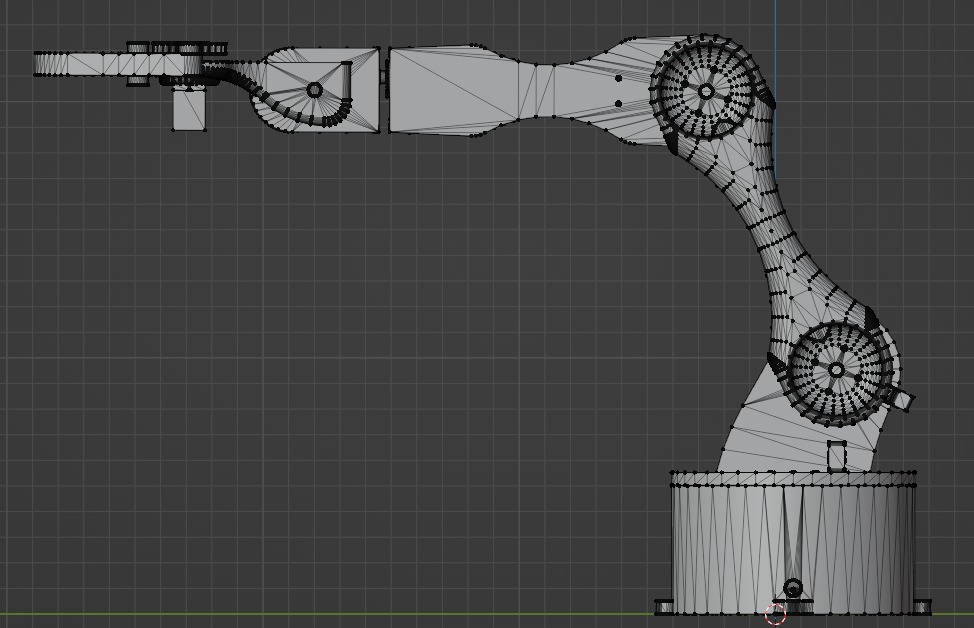
\includegraphics[width=0.75\textwidth]{img/leftW.png}
    \end{center}
    \begin{center}
        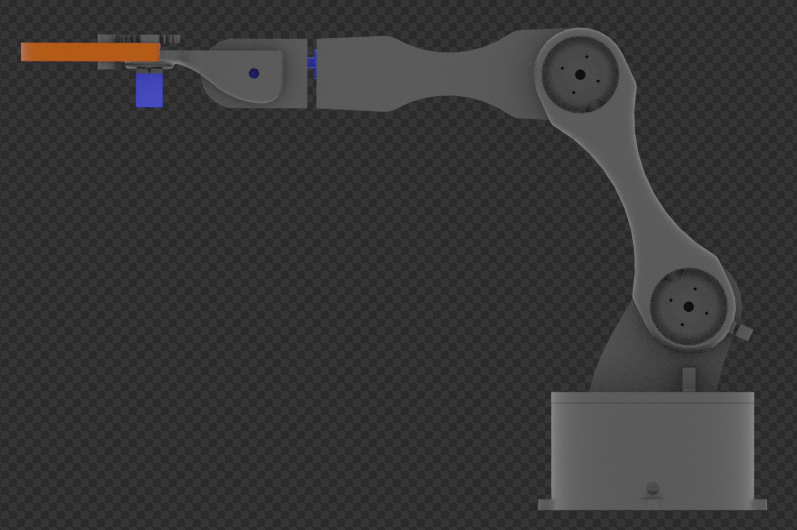
\includegraphics[width=0.75\textwidth]{img/leftC.png}
    \end{center}
    \caption{Proces tworzenia modelu 3D - Widok z boku}
    \label{Modelowanie3Dleft}
\end{figure}

\begin{figure}[p]
    \begin{center}
        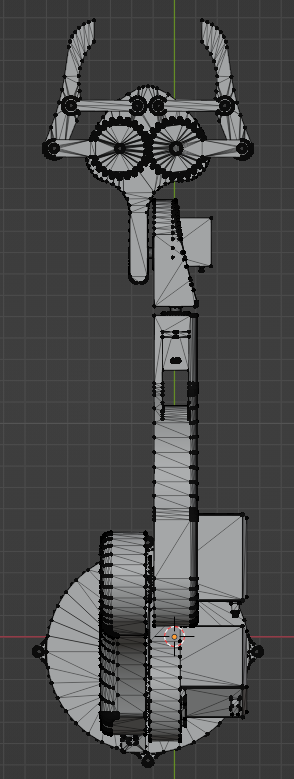
\includegraphics[width=0.4\textwidth]{img/topW.png}
        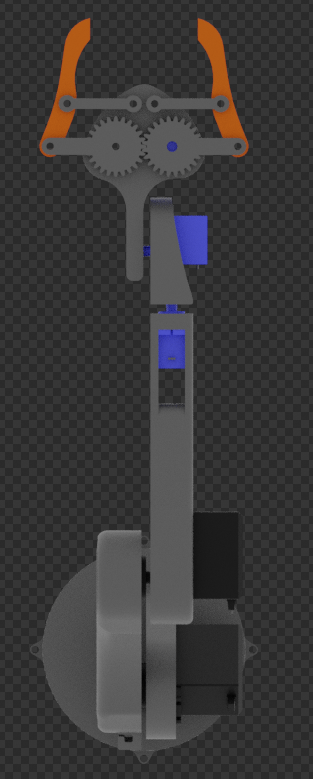
\includegraphics[width=0.4\textwidth]{img/topC.png}
    \end{center}
    \caption{Proces tworzenia modelu 3D - Widok z góry}
    \label{Modelowanie3Dtop}
\end{figure}

\begin{figure}[p]
    \vspace{1cm}
    \begin{center}
        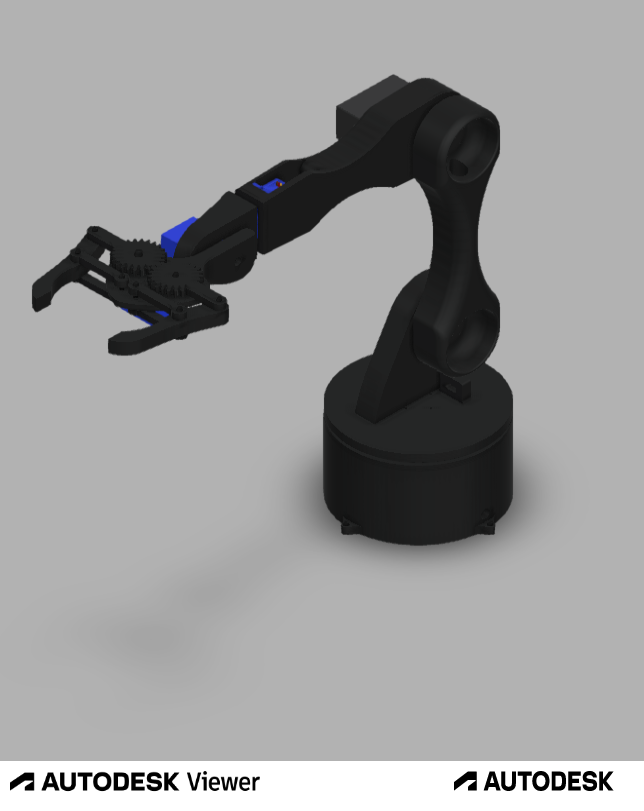
\includegraphics[width=\textwidth]{img/Robak v25.f3d.png}
    \end{center}
    \caption{
        Gotowy model w programie
        \href{https://viewer.autodesk.com/}
        {\underline{Autodesk Viewer}} \\ Narzędzie online do wyświetlania plików 2D i 3D}
    \label{AutodeskViewer}
\end{figure}

\newpage

\subsubsection{\textcolor{blue}{DONE?} Konstrukcja mechaniczna}

Model złożono przy użyciu śrub, wkrętów i nakrętek M3, co przedstawiono na Rysunkach \ref{mechC} i \ref{mechB}.

\begin{figure}[h!]
    \begin{center}
        \includegraphics[width=\textwidth]{img/mechC.jpg}
    \end{center}
    \caption{Konstrukcja mechaniczna - chwytak}
    \label{mechC}
\end{figure}

\begin{figure}[h!]
    \begin{center}
        \includegraphics[width=\textwidth]{img/mechB.jpg}
    \end{center}
    \caption{Konstrukcja mechaniczna - podstawa}
    \label{mechB}
\end{figure}

\subsubsection{\textcolor{blue}{DONE?} Schemat elektryczny}

Na Rysunku \ref{SchematElektryczny}\footnote{Stworzono przy użyciu \href{https://www.circuito.io}{\underline{circuito.io}}} przedstawiono połączenie elementów elektronicznych. Natomiast faktyczne połączenia elektryczne pokazano na Rysunku \ref{Breadboard}.

\vspace{4cm}

\begin{figure}[h!]
    \begin{center}
        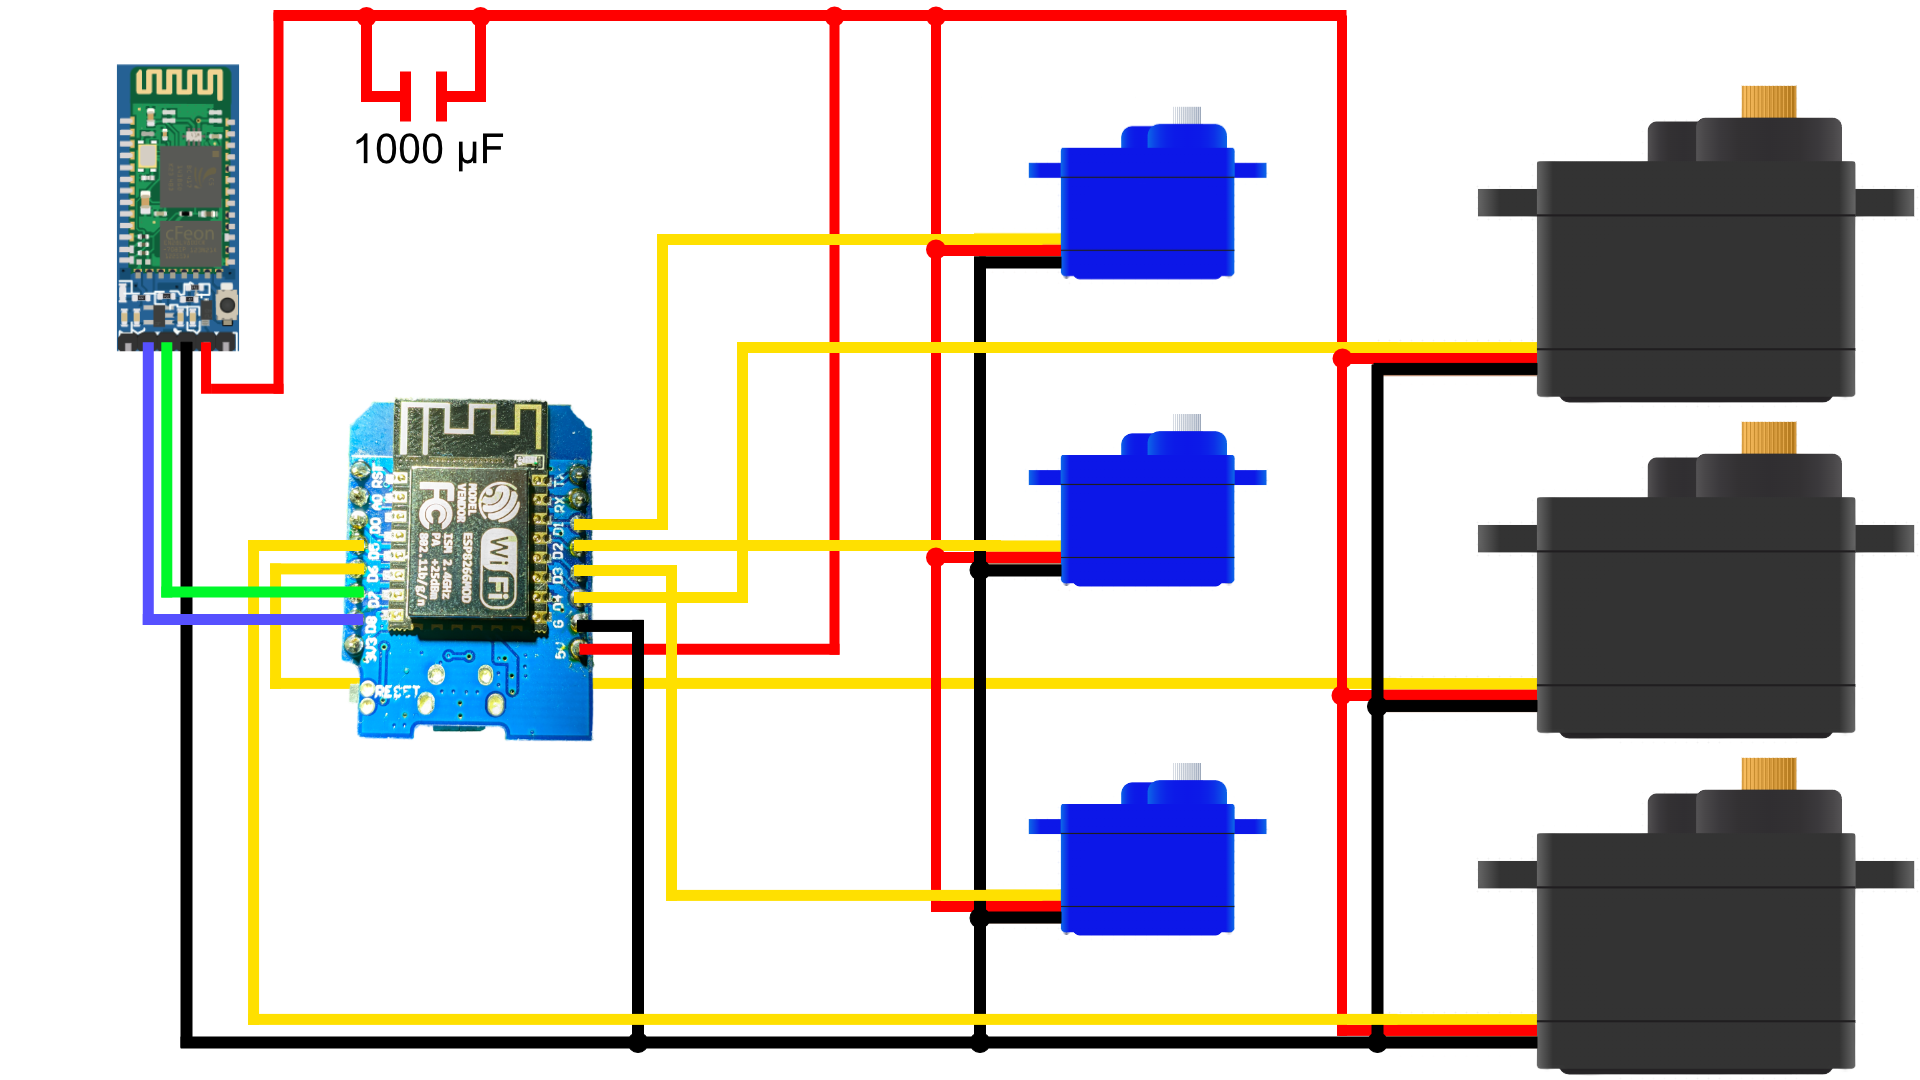
\includegraphics[width=\textwidth]{img/schemat.png}
    \end{center}
    \caption{Schemat połączeń elektrycznych}
    \vspace{4cm}
    \label{SchematElektryczny}
\end{figure}

\begin{figure}[p]
    \begin{center}
        \includegraphics[width=\textwidth]{img/breadboard.jpg}
    \end{center}
    \caption{Połączenia elektryczne}
    \label{Breadboard}
\end{figure}

\subsubsection{\textcolor{blue}{DONE?} Aplikacja}

Aplikacja powstała w \href{https://appinventor.mit.edu}{\underline{MIT App Inventor}}\footnote{Zintegrowane środowisko programistyczne do tworzenia aplikacji mobilnych} (Rysunki \ref{MITapp} i \ref{MITblocks}). Środowisko to oferuje prostotę w realizacji projektów. Nie wymaga żadnego doświadczenia od użytkownika. Programowanie odbywa się we własnym języku graficznym (duże podobieństwo do \href{https://scratch.mit.edu}{\underline{Scratch}}\footnote{Interpretowany wizualny język programowania}). Kod dostarczonej aplikacji pokazano na Załącznikach \ref{AppBluetooth}, \ref{AppPrzyciski}, \ref{AppSlidery} i \ref{AppKomendy}. Na Rysunku \ref{FinalApp} przedstawiono ostateczną szatę graficzną aplikacji.

\begin{figure}[h!]
    \begin{center}
        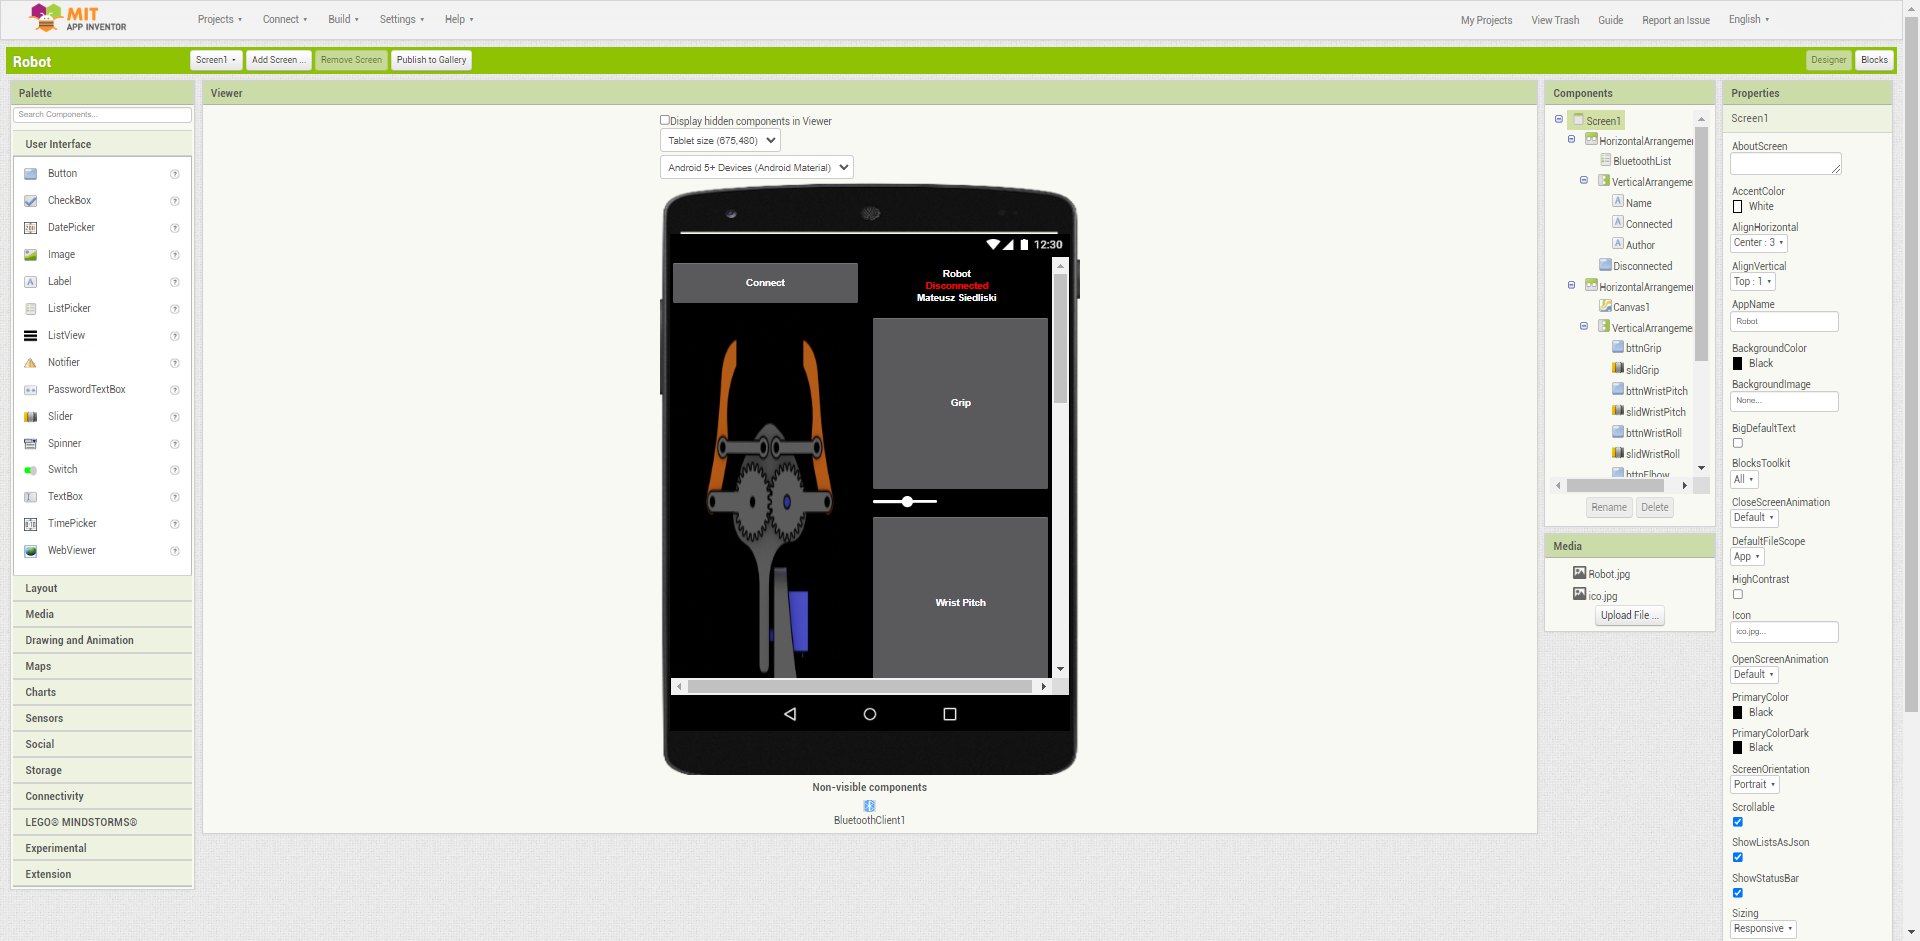
\includegraphics[width=0.8\textwidth]{img/app_src/MITapp.png}
    \end{center}
    \caption{MIT App Inventor - aplikacja}
    \label{MITapp}
\end{figure}

\begin{figure}[h!]
    \begin{center}
        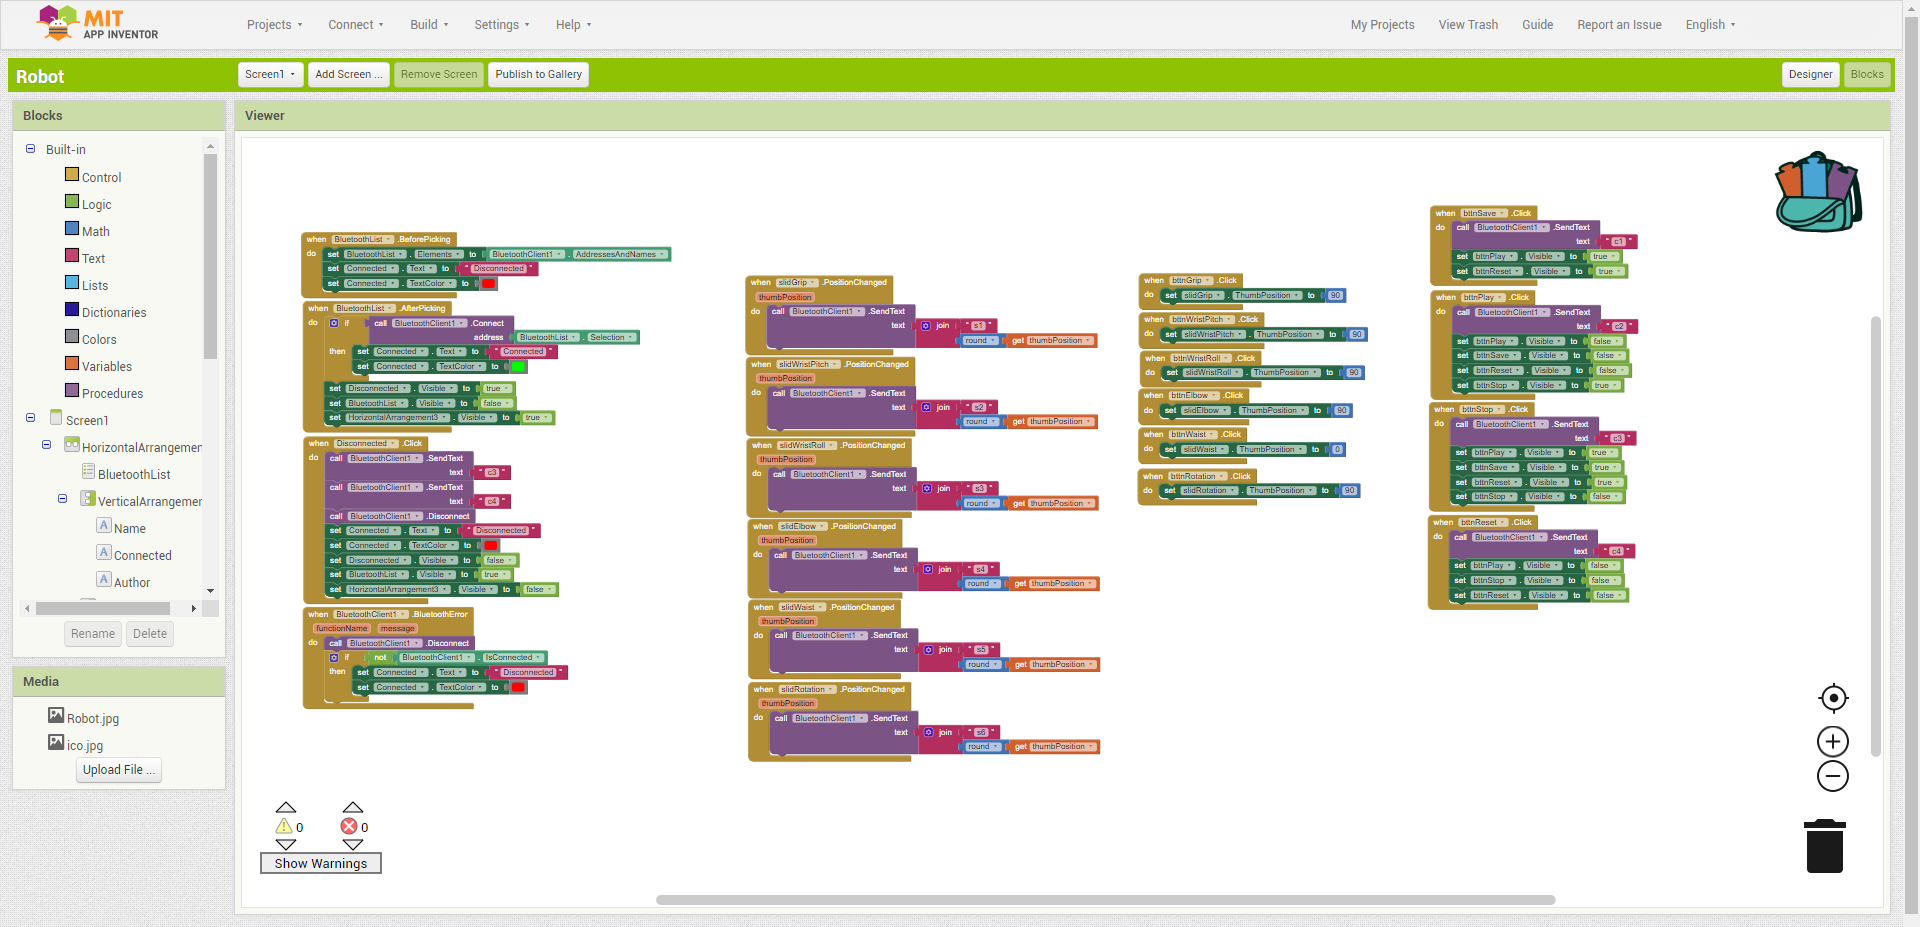
\includegraphics[width=0.8\textwidth]{img/app_src/MITblocks.png}
    \end{center}
    \caption{MIT App Inventor - kod}
    \label{MITblocks}
\end{figure}

\begin{figure}[p]
    \begin{center}
        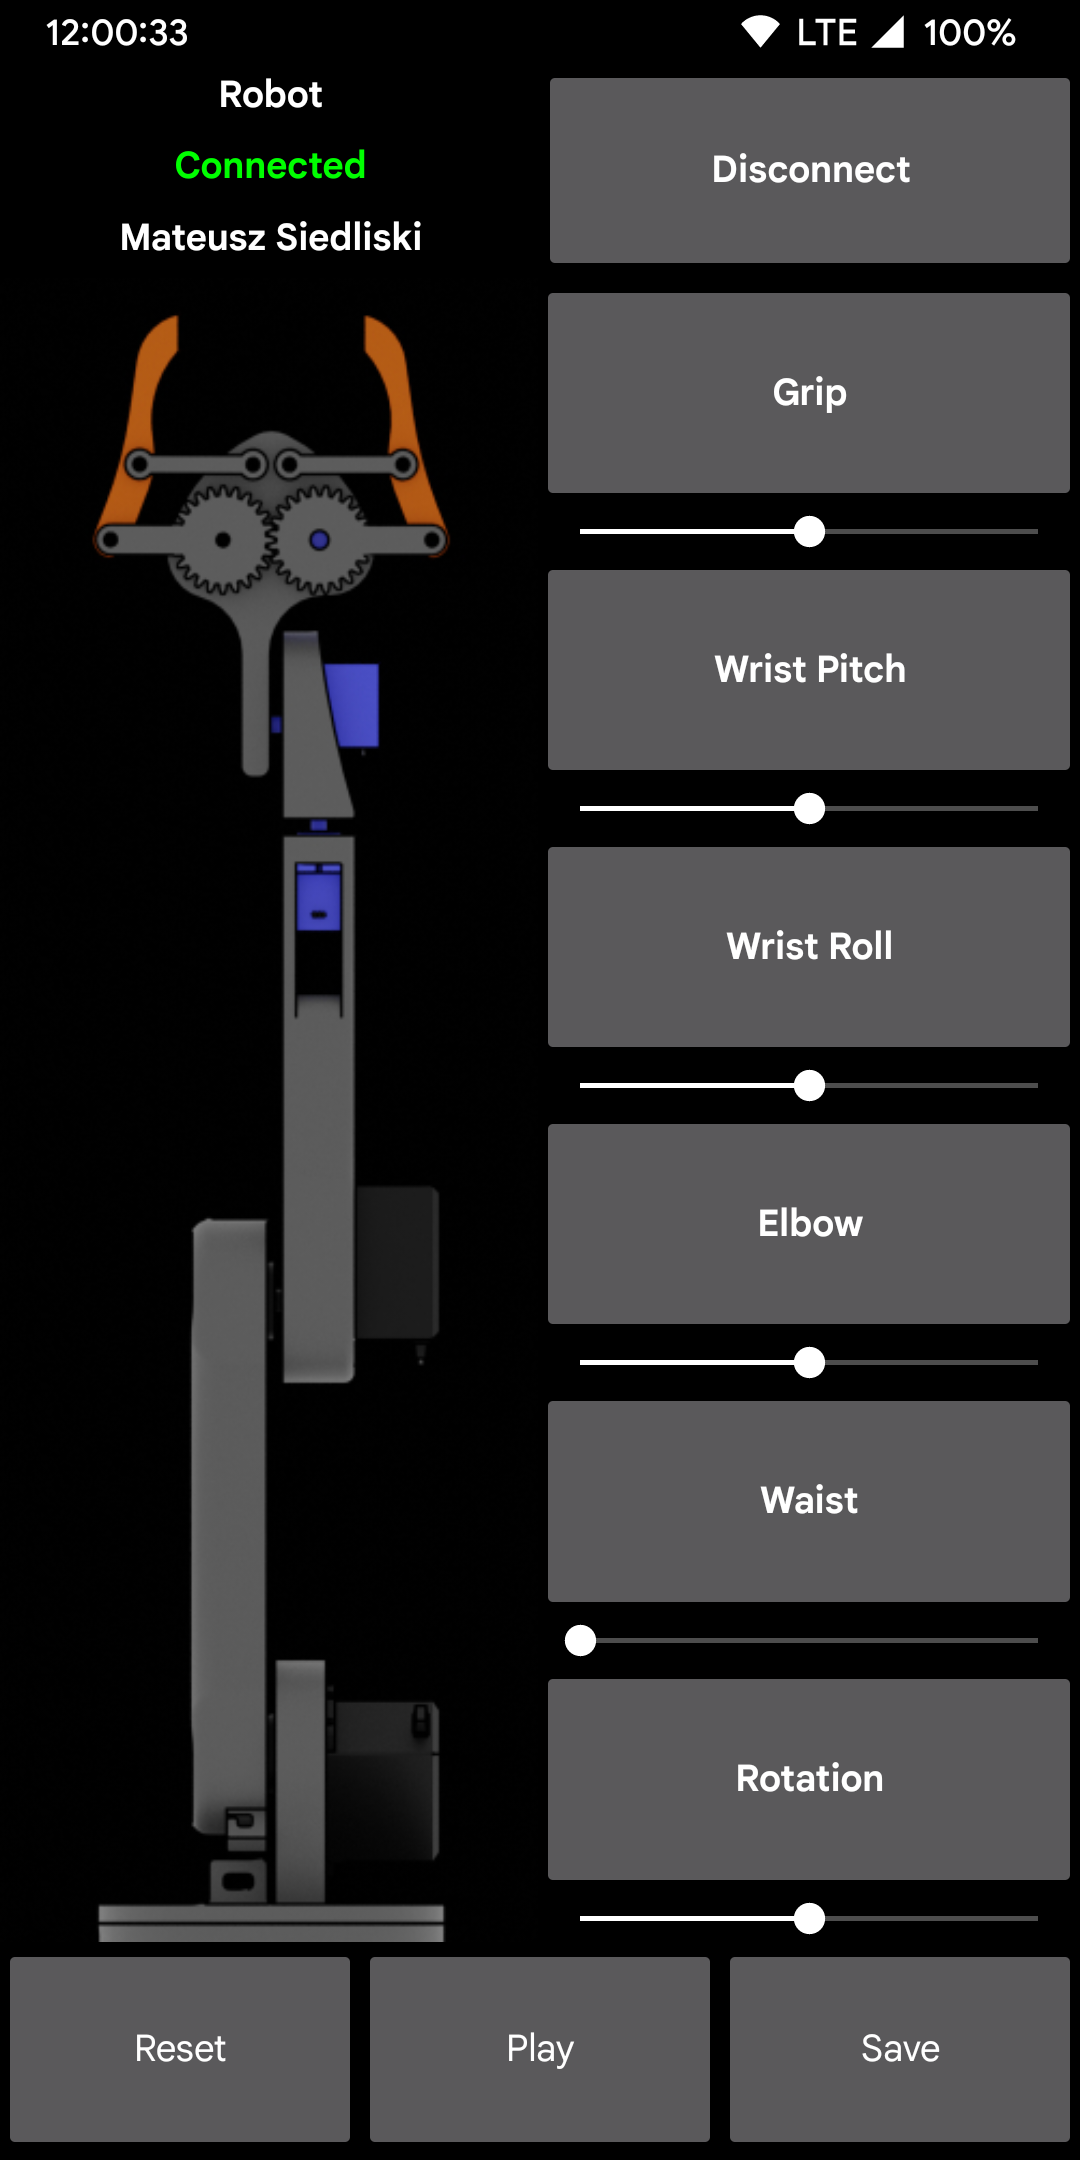
\includegraphics[width=0.8\textwidth]{img/app.png}
    \end{center}
    \caption{Gotowa aplikacja}
    \label{FinalApp}
\end{figure}

\subsubsection{\textcolor{blue}{DONE?} Protokół komunikacyjny}

Komunikacja aplikacji mobilnej z mikrokontrolerem odbywa się poprzez protokół Bluetooth przy użyciu modułu HC-05. Każdy komunikat to odpowiednio sformatowany string. Komendy komunikacyjne przedstawiono w Tabeli \ref{Komunikacja}. Przykładowe komunikaty:
\begin{itemize}
    \item \enquote{s1128\textbackslash0} - ustawienie serwomechanizmu 1 na pozycję 128
    \item \enquote{s564\textbackslash0} - ustawienie serwomechanizmu 5 na pozycję 64
    \item \enquote{c1\textbackslash0} - zapisanie aktualnej pozycji serwomechanizmów w pamięci do późniejszego odtworzenia
    \item \enquote{c4\textbackslash0} - wyczyszczenie zapisanej sekwencji ruchowej
\end{itemize}

\vspace{2cm}

\begin{table}[h!]
    \begin{center}
        \begin{tabular}{|c|c|c|m{8cm}|}
            \hline
            Komenda & Numer & Wartość & Funkcja                                                                                   \\
            \hline
            s       & 1     & x       & Ustawienie serwomechanizmu na pozycję x                                                   \\
            \hline
            s       & 2     & x       & Ustawienie serwomechanizmu na pozycję x                                                   \\
            \hline
            s       & 3     & x       & Ustawienie serwomechanizmu na pozycję x                                                   \\
            \hline
            s       & 4     & x       & Ustawienie serwomechanizmu na pozycję x                                                   \\
            \hline
            s       & 5     & x       & Ustawienie serwomechanizmu na pozycję x                                                   \\
            \hline
            s       & 6     & x       & Ustawienie serwomechanizmu na pozycję x                                                   \\
            \hline
            c       & 1     & -       & Save - zapisanie aktualnej pozycji serwomechanizmów w pamięci do późniejszego odtworzenia \\
            \hline
            c       & 2     & -       & Play - odtworzanie zapisanej sekwencji ruchowej                                           \\
            \hline
            c       & 3     & -       & Stop - koniec odtwarzania zapisanej sekwencji ruchowej                                    \\
            \hline
            c       & 4     & -       & Reset - wyczyszczenie zapisanej sekwencji ruchowej                                        \\
            \hline
        \end{tabular}
    \end{center}
    \caption{Protokół komunikacyjny}
    \label{Komunikacja}
\end{table}

\newpage

\subsubsection{\textcolor{blue}{DONE?} Kod mikrokontrolera}

Kod sterujący działaniem mikrokontrolera powstał w \href{https://code.visualstudio.com}{\underline{Visual Studio Code}}\footnote{Darmowy edytor kodu źródłowego z kolorowaniem składni dla wielu języków, stworzony przez Microsoft o otwartym kodzie źródłowym} przy pomocy \href{https://platformio.org}{\underline{PlatformIO}}\footnote{\enquote{A user-friendly and extensible integrated development environment with a set of professional development instruments, providing modern and powerful features to speed up yet simplify the creation and delivery of embedded products}\cite{platformio}}. Schemat blokowy kodu przedstawiono na rysunku \ref{SBCode}\footnote{Schemat wykonano w programie \href{https://www.lucidchart.com}{\underline{Lucidchart}}}. Całość kodu źródłowego znajduje się w Załączniku \ref{KodMikrokontrolera}.

\vspace{1cm}

\begin{figure}[h!]
    \begin{center}
        \includesvg[width=0.7\textwidth]{img/schematkodu.svg}
    \end{center}
    \caption{Schemat blokowy kodu}
    \label{SBCode}
\end{figure}

W celu ograniczenia prędkości poruszania się każdego z serwomechanizmów zastosowano funkcję przedstawioną na Rysunku \ref{void_moveServo}. Wykonuje ona swoje zadanie poprzez iteracyjną inkrementację lub dekrementację wartości pozycji.

\vspace{1cm}

\begin{figure}[h!]
    \lstinputlisting[firstline=152,lastline=182]{../src/main.cpp}
    \caption{void moveServo()}
    \label{void_moveServo}
\end{figure}

\newpage

Innym ciekawym rozwiązaniem jest realizacja odtwarzania zapisanej sekwencji ruchów, które pokazano na Rysunku \ref{casePlay}. Rozwiązanie polega na iteracyjnej inkrementacji bądź dekrementacji wartości pozycji dla wszystkich serwomechanizmów po kolei.

\begin{figure}[h!]
    \lstinputlisting[firstline=109,lastline=142]{../src/main.cpp}
    \caption{case 2: - Play}
    \label{casePlay}
\end{figure}

Nieocenioną pomocą okazały się biblioteki:
\begin{itemize}
    \item Arduino.h \cite{Arduino_lib}
    \item SoftwareSerial.h \cite{EspSoftwareSerial}
    \item Servo.h \cite{EspServo}
\end{itemize}

\subsection{\textcolor{orange}{TODO} Problemy w trakcie tworzenia sprzętu i aplikacji}

W tym punkcie należy przedstawić jakie były problemy przed którymi stanęli autorzy projektu w trakcie jego realizacji i jak je rozwiązali.

\newpage

\section{\textcolor{orange}{TODO} Podsumowanie}

W ostatnim punkcie opisać co zostało wykonane, jakiej części założeń nie wykonano i dlaczego. Co można zrobić, by dany projekt poprawić i w jakim kierunku może pójść dalszy rozwój tego projektu.

\newpage

\section{\textcolor{red}{WIP}  Literatura}

\printbibliography[heading=none]

\newpage

\section{\textcolor{red}{WIP} Załączniki}

Na prezentację (obronę) projektu trzeba przygotować prezentację w PowerPoint lub Prezi trwającą ok 12-15 minut Zwykle jest to ok. 20 slajdów. Te slajdy muszą zawierać tytuł projektu, autora, prowadzącego. Następnie plan prezentacji, najważniejsze osiągnięcia , podsumowanie. Slajdy muszą być czytelne, należy umieszczać rysunki i schematy, także nie powinno się na nich umieszczać zbyt dużo tekstu (tekst powinien mieć ok. 20-24pkt). W trakcie lub po prezentacji powinno się zademonstrować wykonany sprzęt i oprogramowanie. Można również zaprezentować w zamian tego film z działania urządzenia.

Przykładowa zawartość załącznika:
Kody źródłowe (z komentarzami!!!) na CD spakowane.
Wysłane mailem zawartość projektu do prowadzącego.
Prezentacja.
Wszystkie opisy układów, programów, narzędzi stosowanych w projekcie itp.

\newpage

\renewcommand*{\lstlistingname}{Załącznik}
\renewcommand*{\figurename}{Załącznik}
\setcounter{figure}{1}

\lstinputlisting[label={KodMikrokontrolera},caption={Kod mikrokontrolera}]{../src/main.cpp}

\begin{figure}[p]
    \begin{center}
        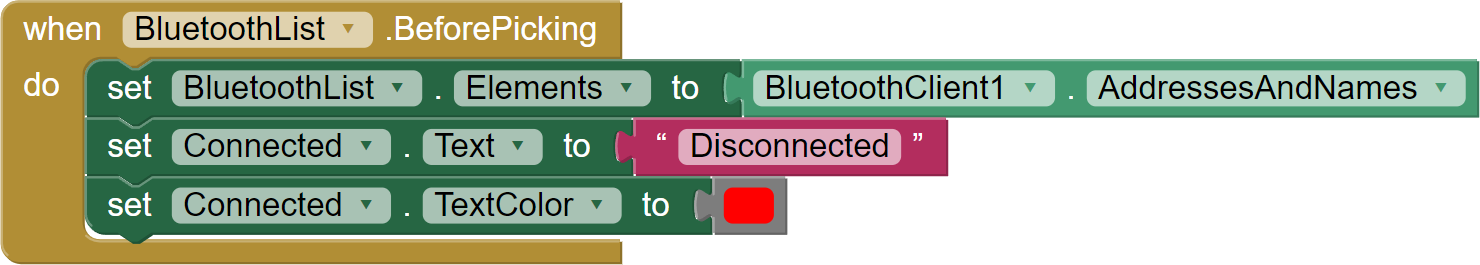
\includegraphics[width=0.8\textwidth]{img/app_src/bluetooth/BluetoothListBefore.png}
        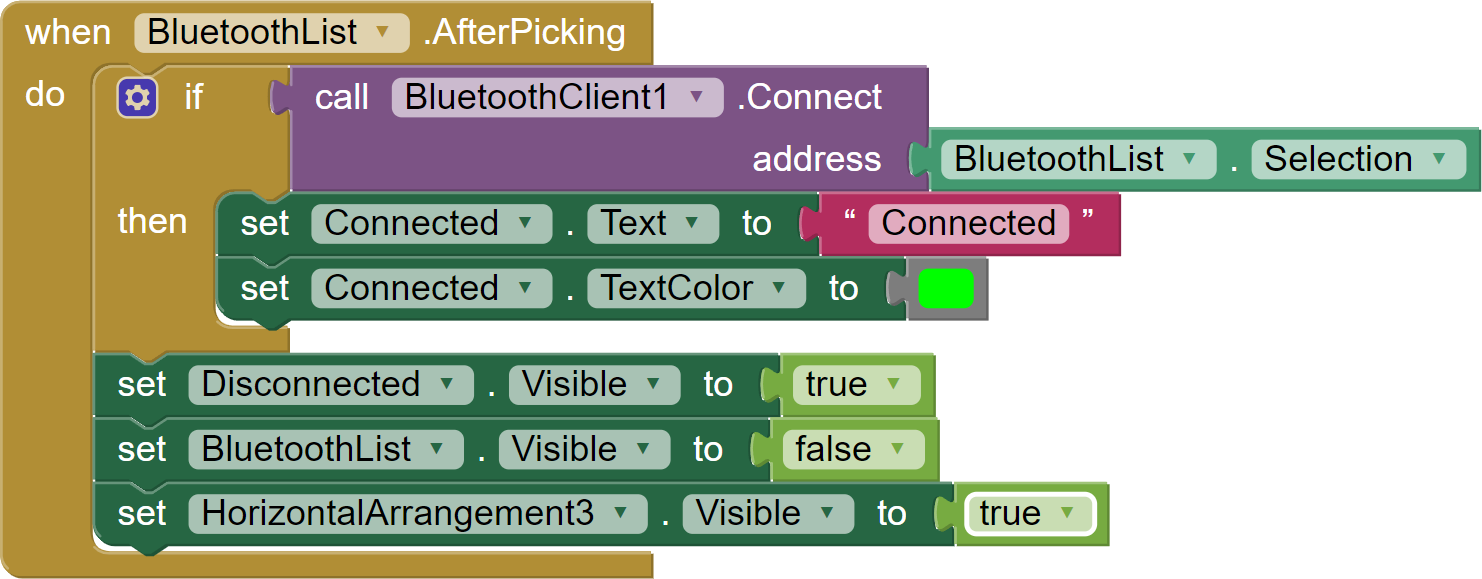
\includegraphics[width=0.8\textwidth]{img/app_src/bluetooth/BluetoothListAfter.png}
        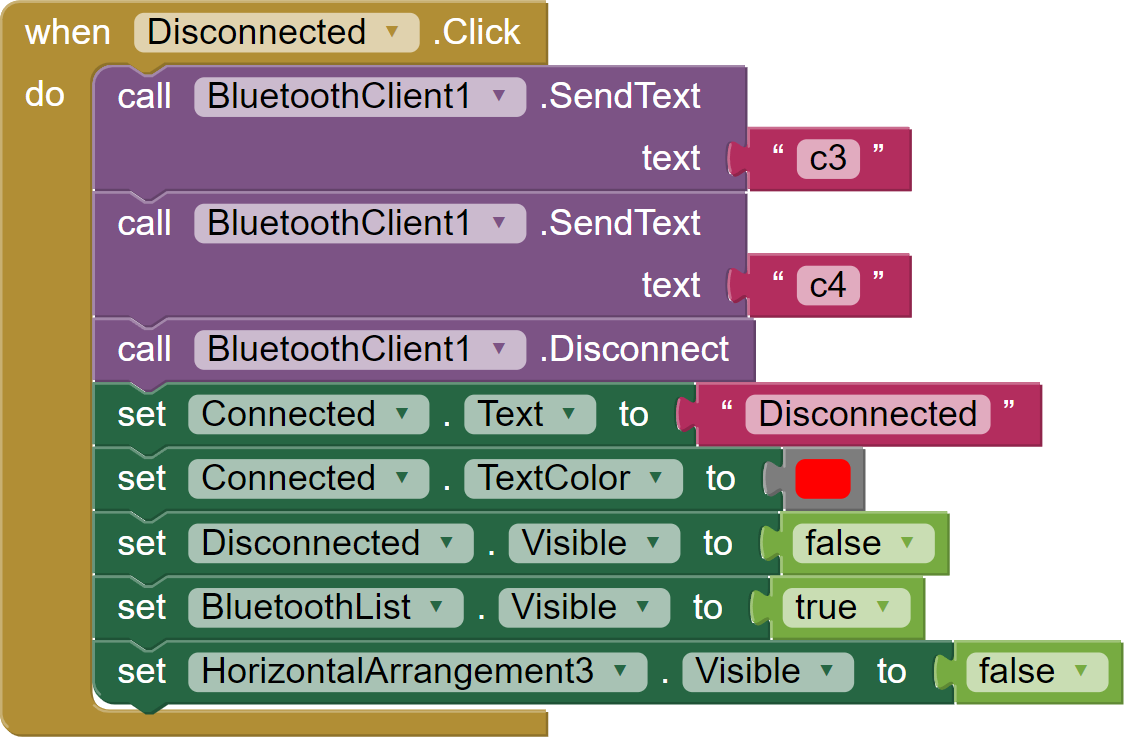
\includegraphics[width=0.8\textwidth]{img/app_src/bluetooth/BluetoothDisconnected.png}
        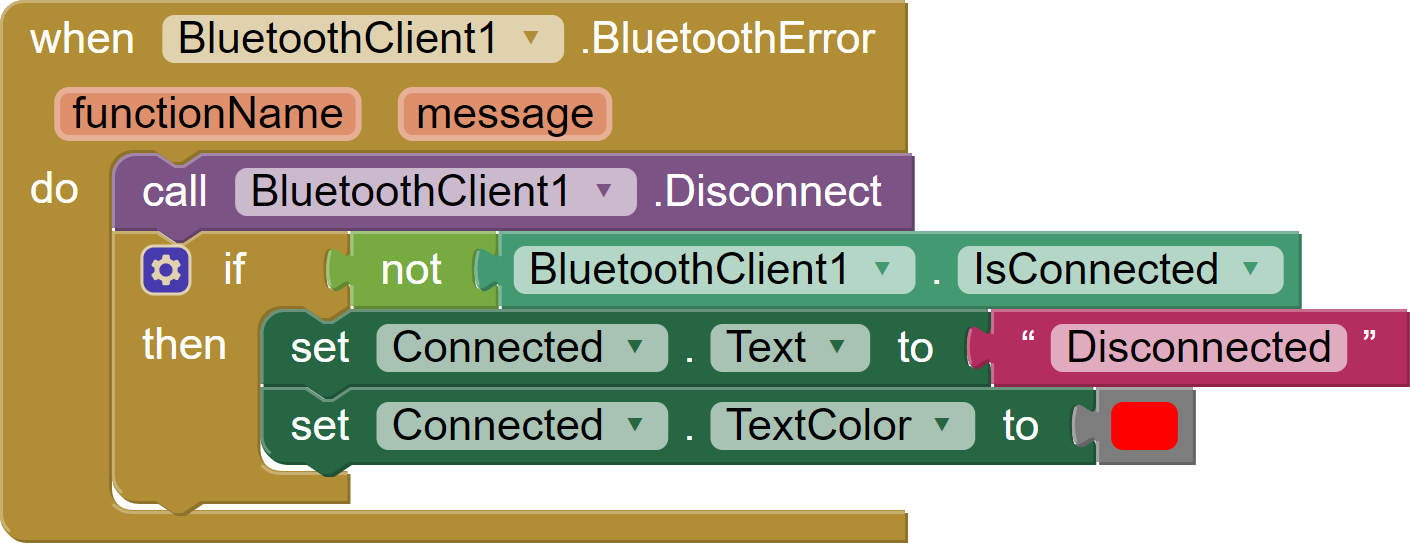
\includegraphics[width=0.8\textwidth]{img/app_src/bluetooth/BluetoothClient.png}
    \end{center}
    \caption{Kod aplikacji - Bluetooth}
    \label{AppBluetooth}
\end{figure}

\newpage

\begin{figure}[p]
    \begin{center}
        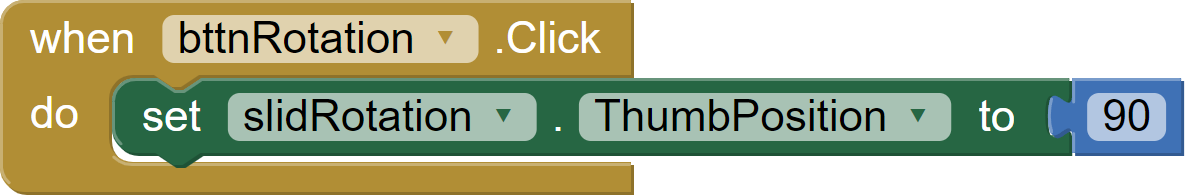
\includegraphics[width=0.9\textwidth]{img/app_src/posButtons/bttnRotation.png}
        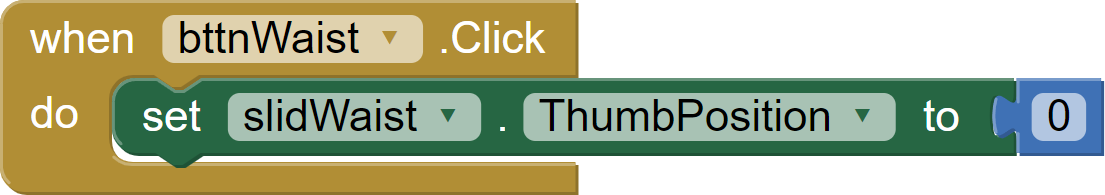
\includegraphics[width=0.9\textwidth]{img/app_src/posButtons/bttnWaist.png}
        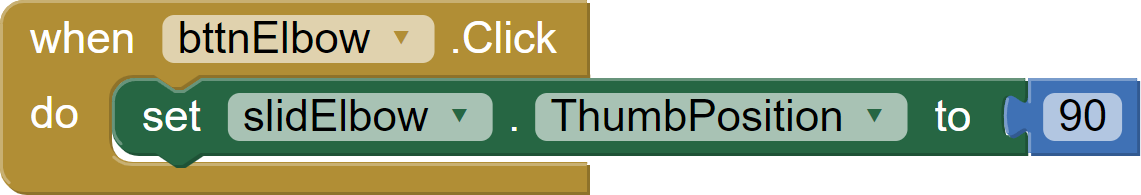
\includegraphics[width=0.9\textwidth]{img/app_src/posButtons/bttnElbow.png}
        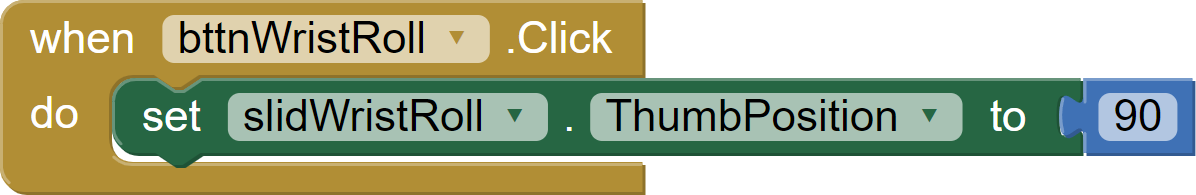
\includegraphics[width=0.9\textwidth]{img/app_src/posButtons/bttnWristRoll.png}
        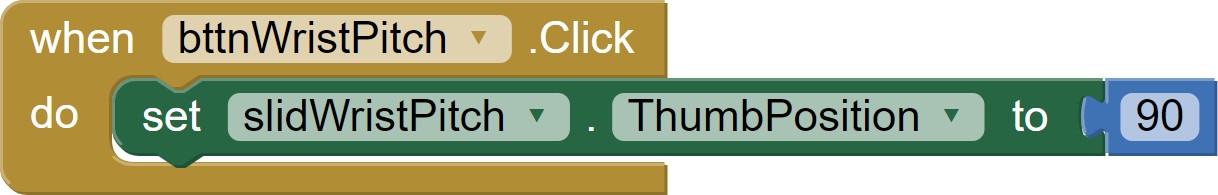
\includegraphics[width=0.9\textwidth]{img/app_src/posButtons/bttnWristPitch.png}
        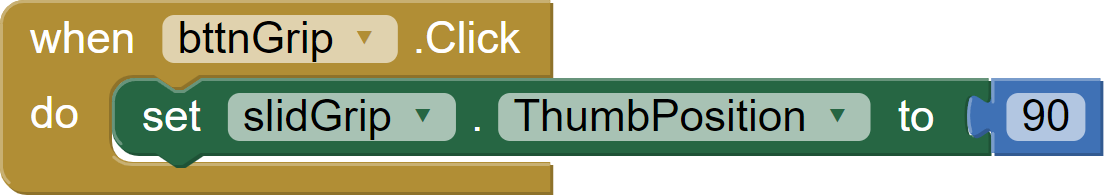
\includegraphics[width=0.9\textwidth]{img/app_src/posButtons/bttnGrip.png}
    \end{center}
    \caption{Kod aplikacji - Przyciski}
    \label{AppPrzyciski}
\end{figure}

\newpage

\begin{figure}[p]
    \begin{center}
        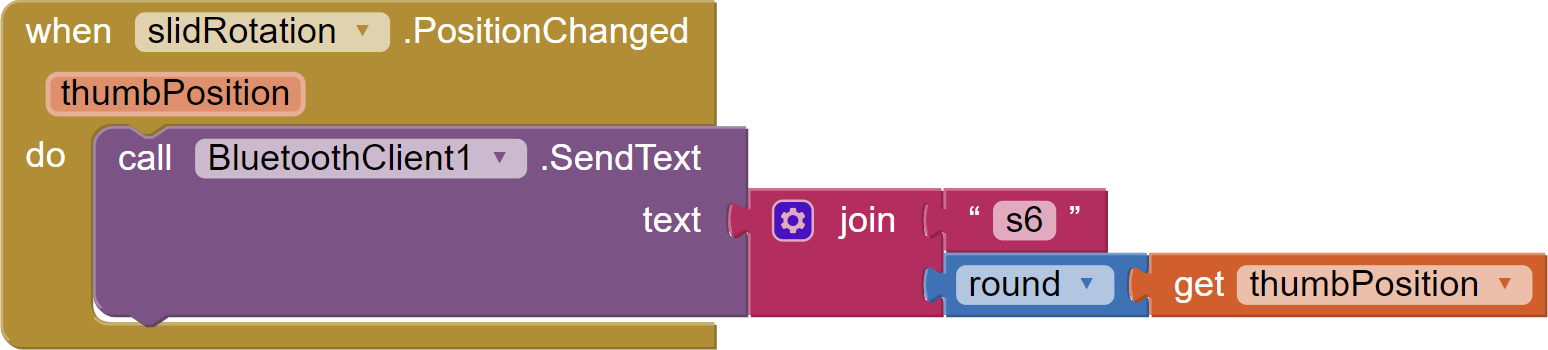
\includegraphics[width=0.9\textwidth]{img/app_src/sliders/slidRotation.png}
        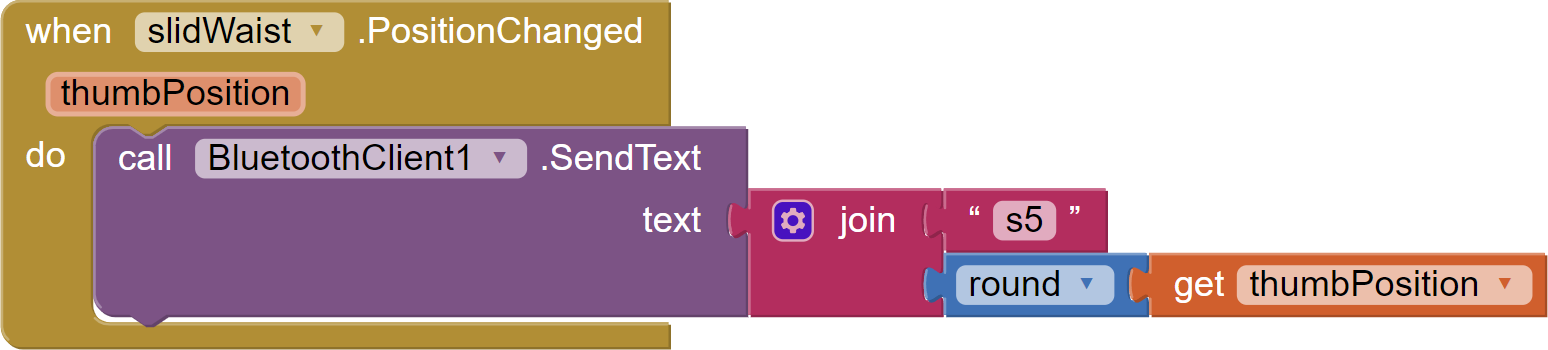
\includegraphics[width=0.9\textwidth]{img/app_src/sliders/slidWaist.png}
        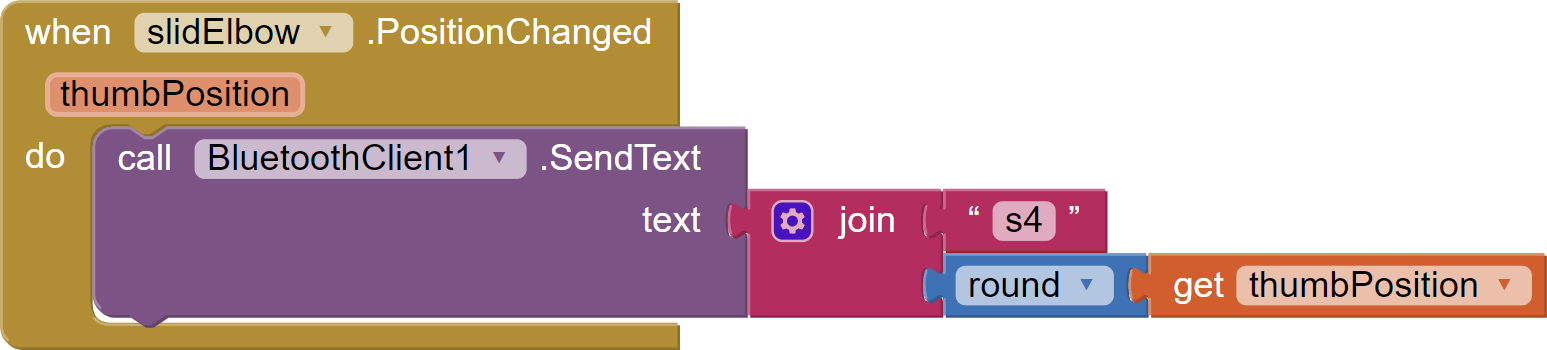
\includegraphics[width=0.9\textwidth]{img/app_src/sliders/slidElbow.png}
        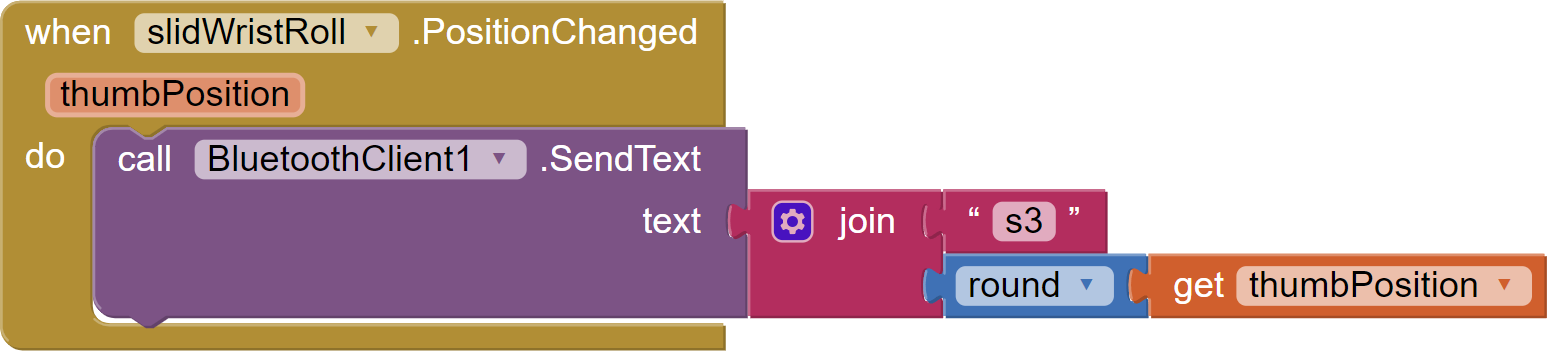
\includegraphics[width=0.9\textwidth]{img/app_src/sliders/slidWristRoll.png}
        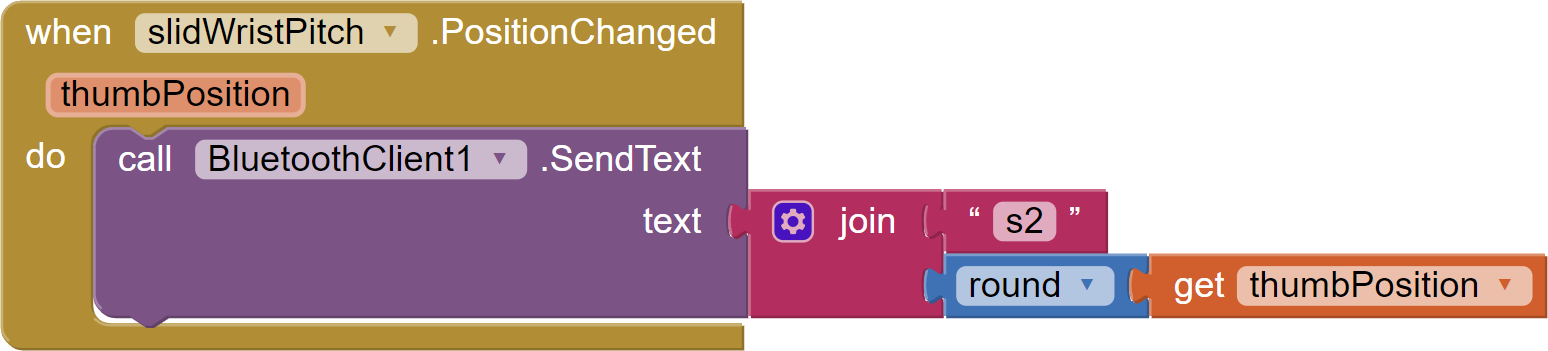
\includegraphics[width=0.9\textwidth]{img/app_src/sliders/slidWristPitch.png}
        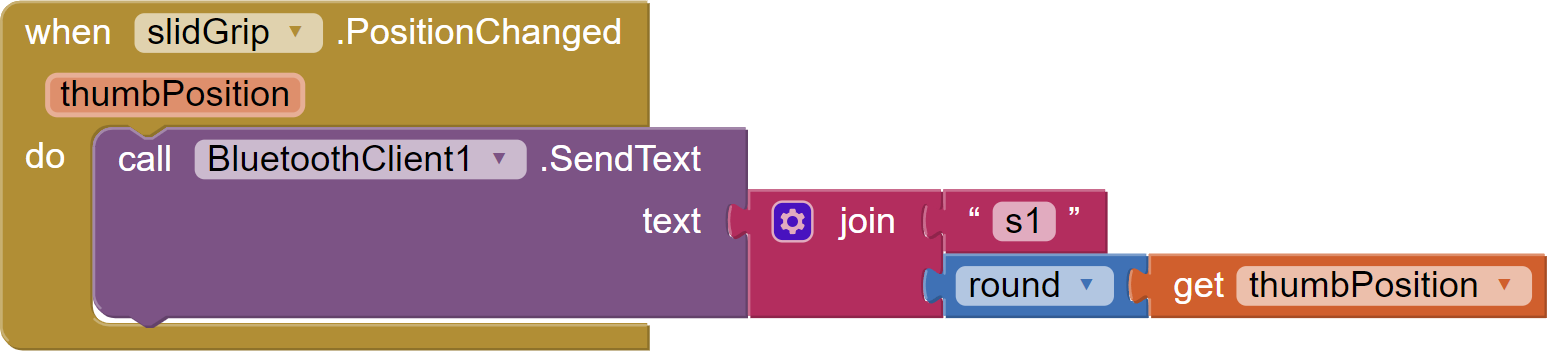
\includegraphics[width=0.9\textwidth]{img/app_src/sliders/slidGrip.png}
    \end{center}
    \caption{Kod aplikacji - Slidery}
    \label{AppSlidery}
\end{figure}

\newpage

\begin{figure}[p]
    \begin{center}
        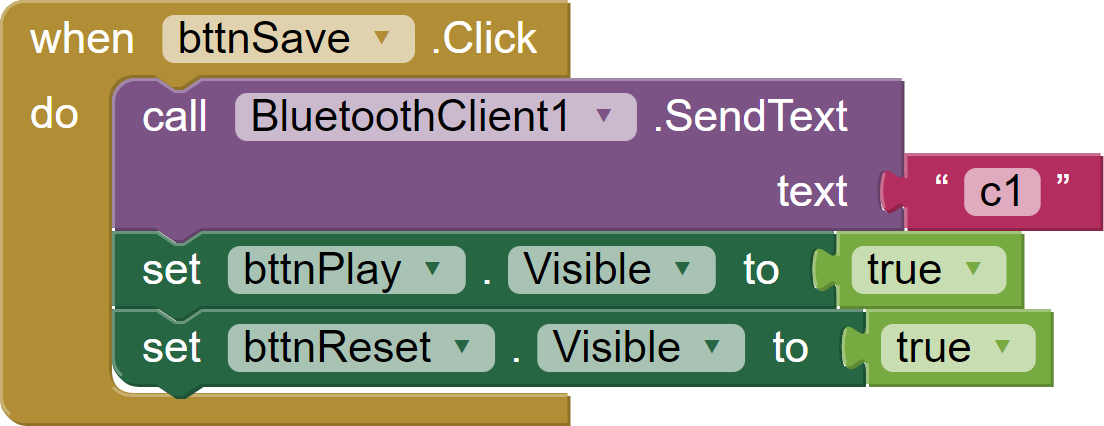
\includegraphics[width=0.8\textwidth]{img/app_src/commands/Save.png}
        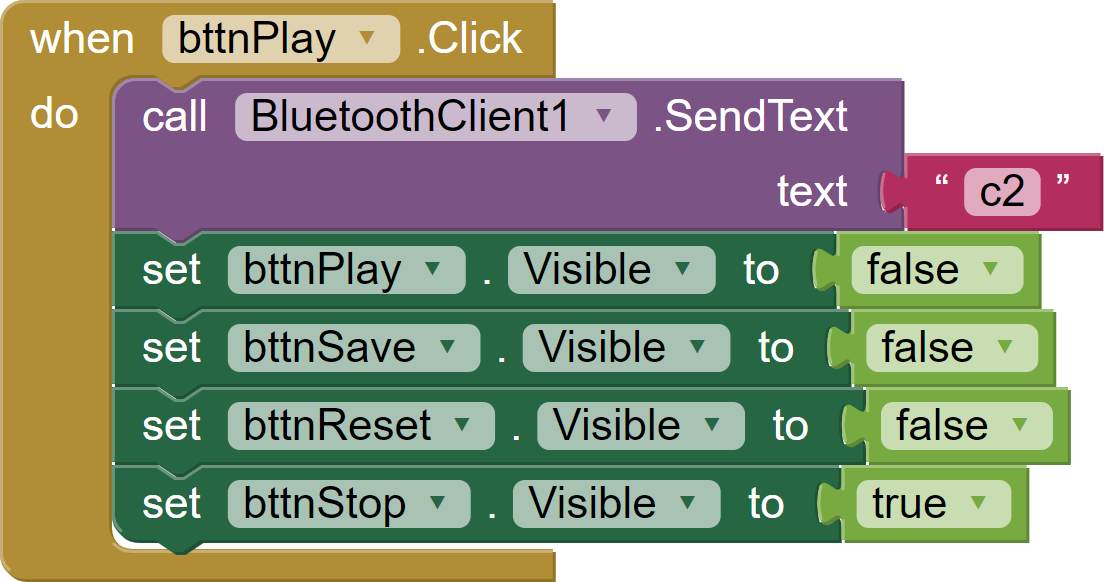
\includegraphics[width=0.8\textwidth]{img/app_src/commands/Play.png}
        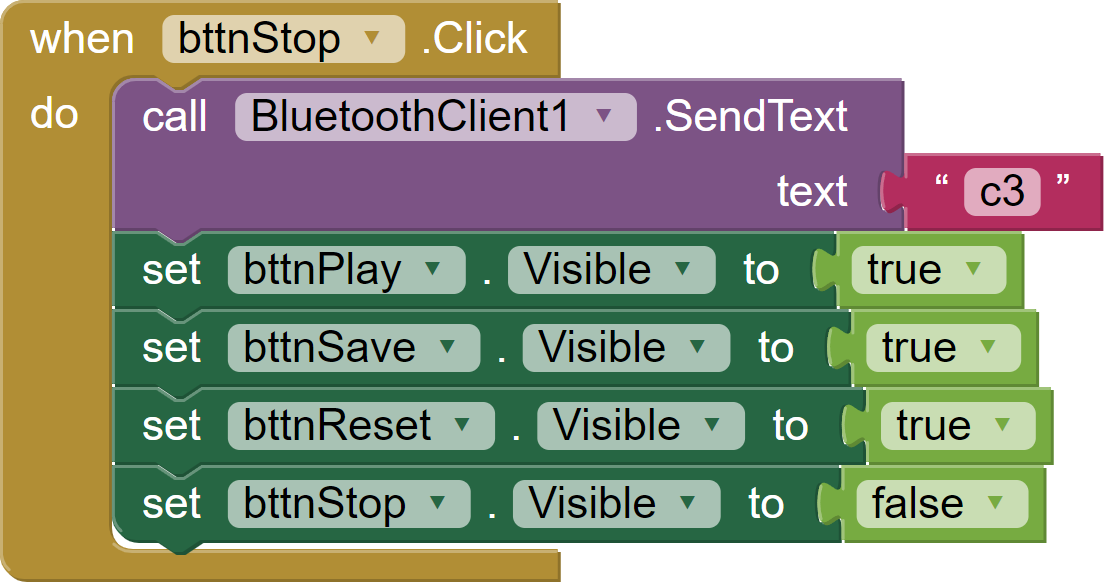
\includegraphics[width=0.8\textwidth]{img/app_src/commands/Stop.png}
        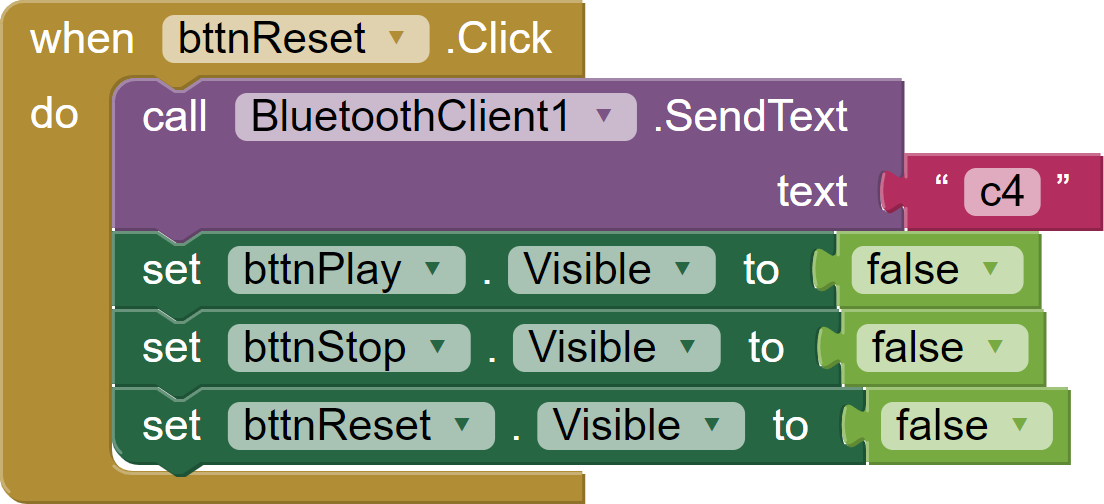
\includegraphics[width=0.8\textwidth]{img/app_src/commands/Reset.png}
    \end{center}
    \caption{Kod aplikacji - Komendy}
    \label{AppKomendy}
\end{figure}

\newpage

\begin{figure}[p]
    \caption{Wemos D1 mini - datasheet}
    \label{wemos}
\end{figure}

\clearpage

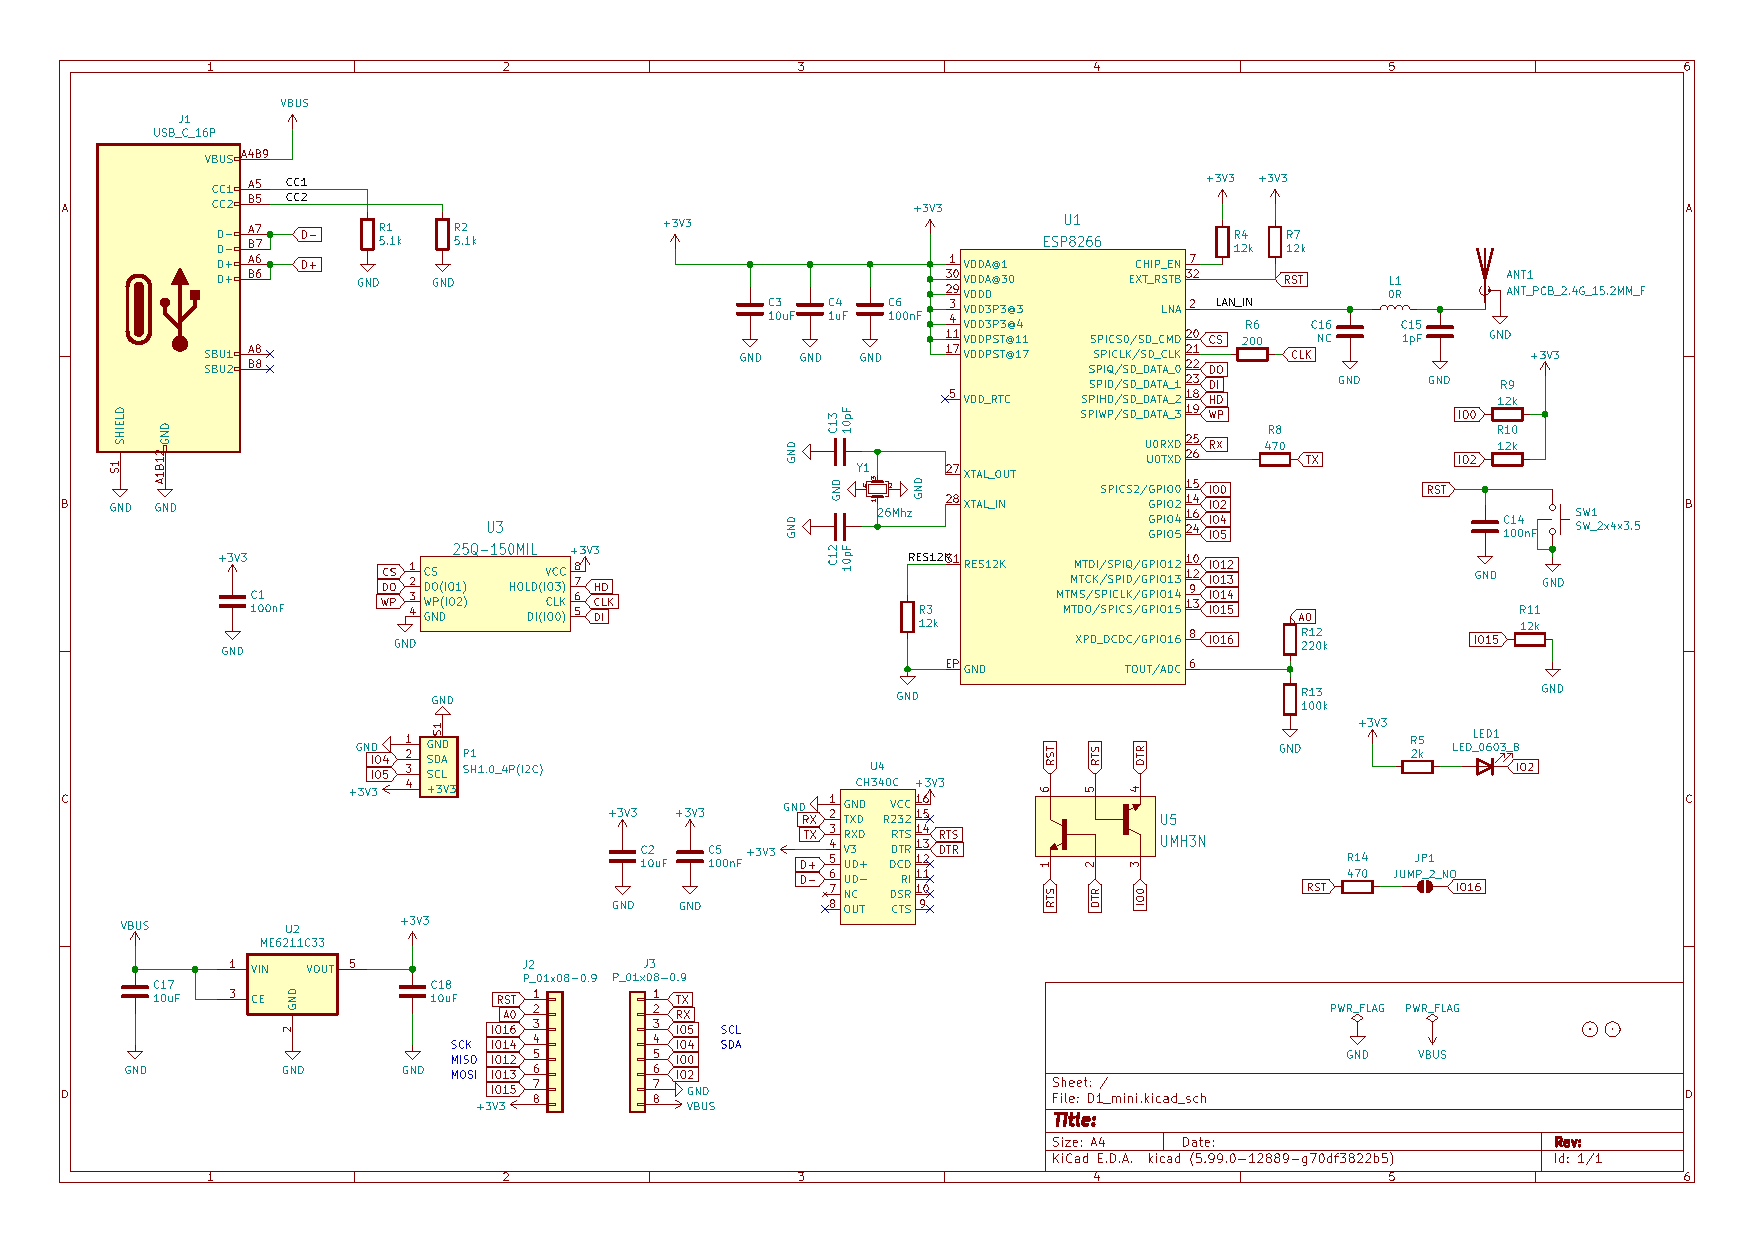
\includepdf[pages=-,fitpaper]{datasheet/sch_d1_mini_v4.0.0.pdf}

\newpage

\begin{figure}[p]
    \caption{HC-05 - datasheet}
    \label{HC05data}
\end{figure}

\clearpage


\includepdf[pages=-,fitpaper]{datasheet/HC-05_datasheet.pdf}

\newpage

\begin{figure}[p]
    \caption{HC-05 - AT}
    \label{HC05at}
\end{figure}

\clearpage

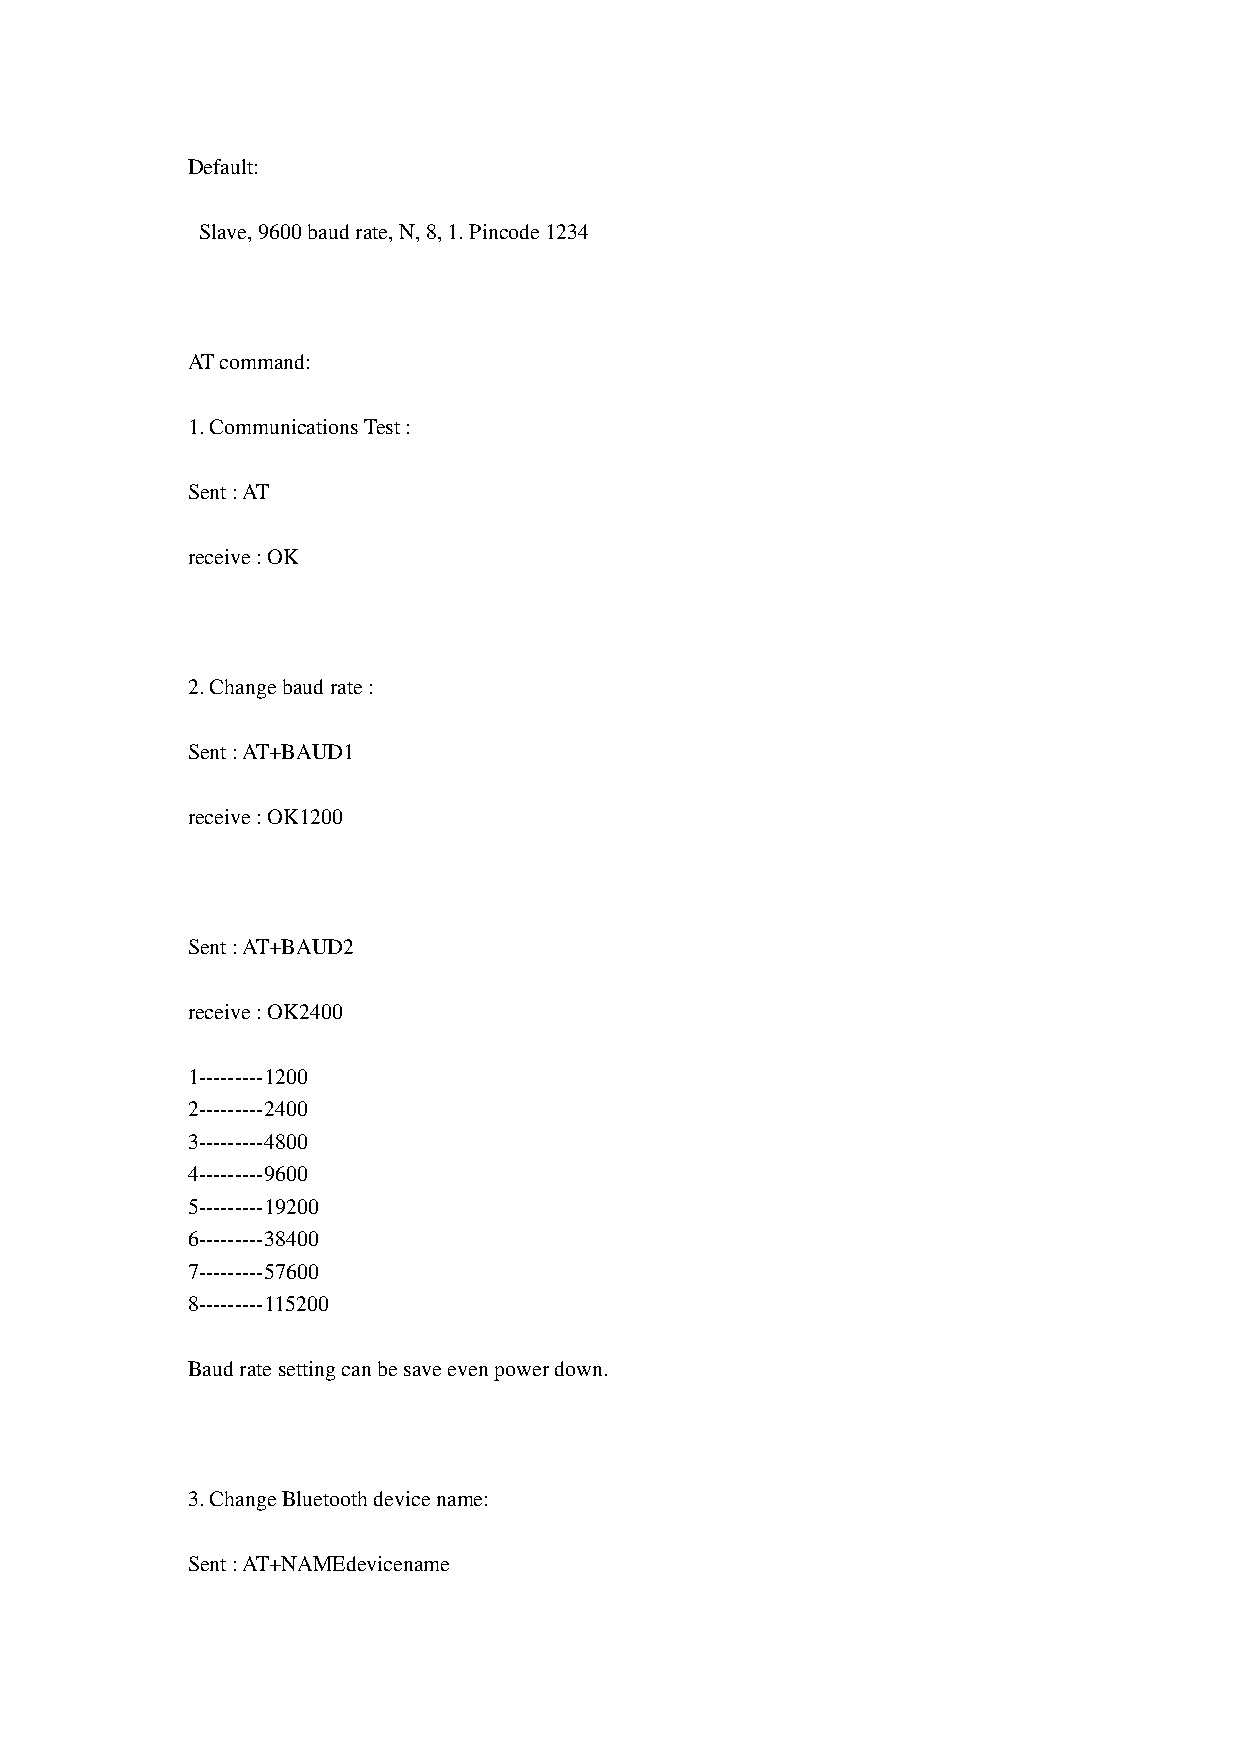
\includepdf[pages=-,fitpaper]{datasheet/HC-05_ATcommands.pdf}

\newpage

\begin{figure}[p]
    \caption{Micro Servo 9g SG90 - datasheet}
    \label{ServoSG90}
\end{figure}

\clearpage

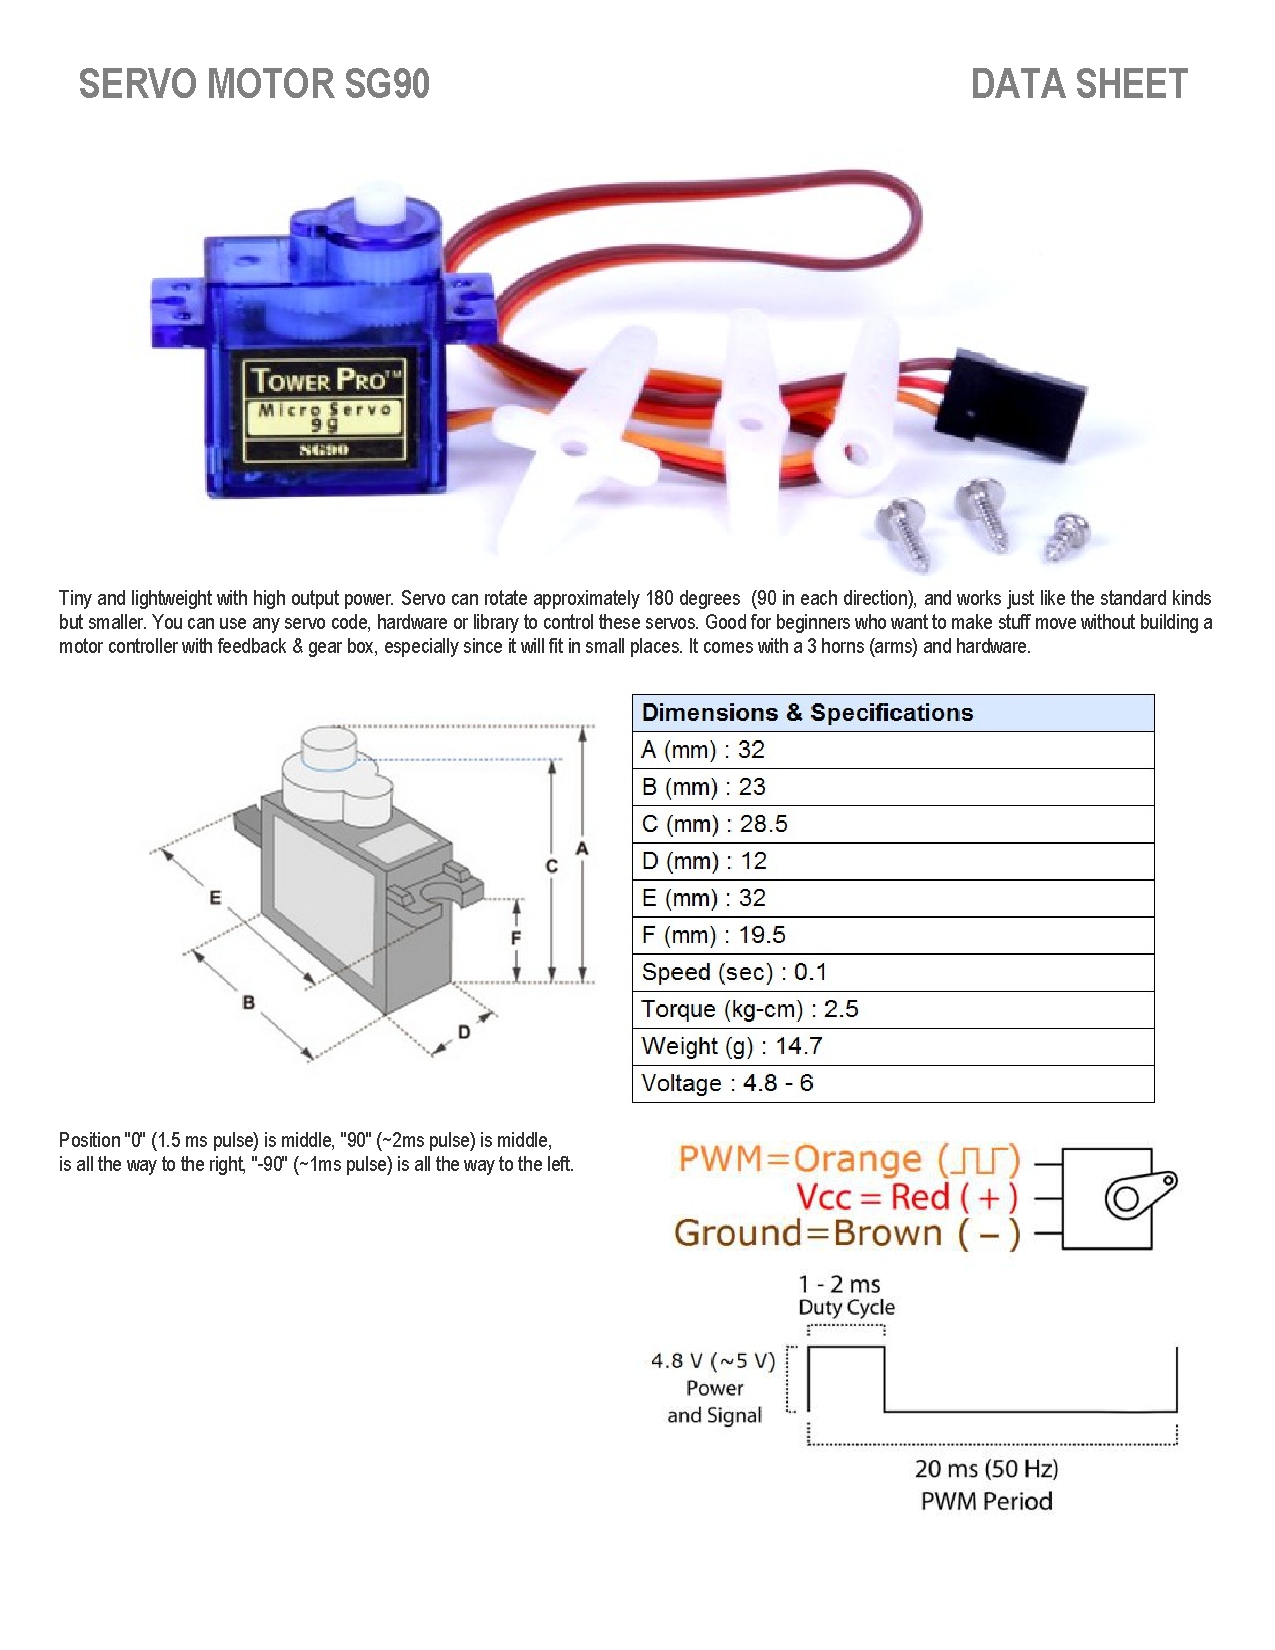
\includepdf[pages=-,fitpaper]{datasheet/sg90_datasheet.pdf}

\newpage

\begin{figure}[p]
    \caption{Servo Mg996r - datasheet}
    \label{ServoMg996r}
\end{figure}

\clearpage

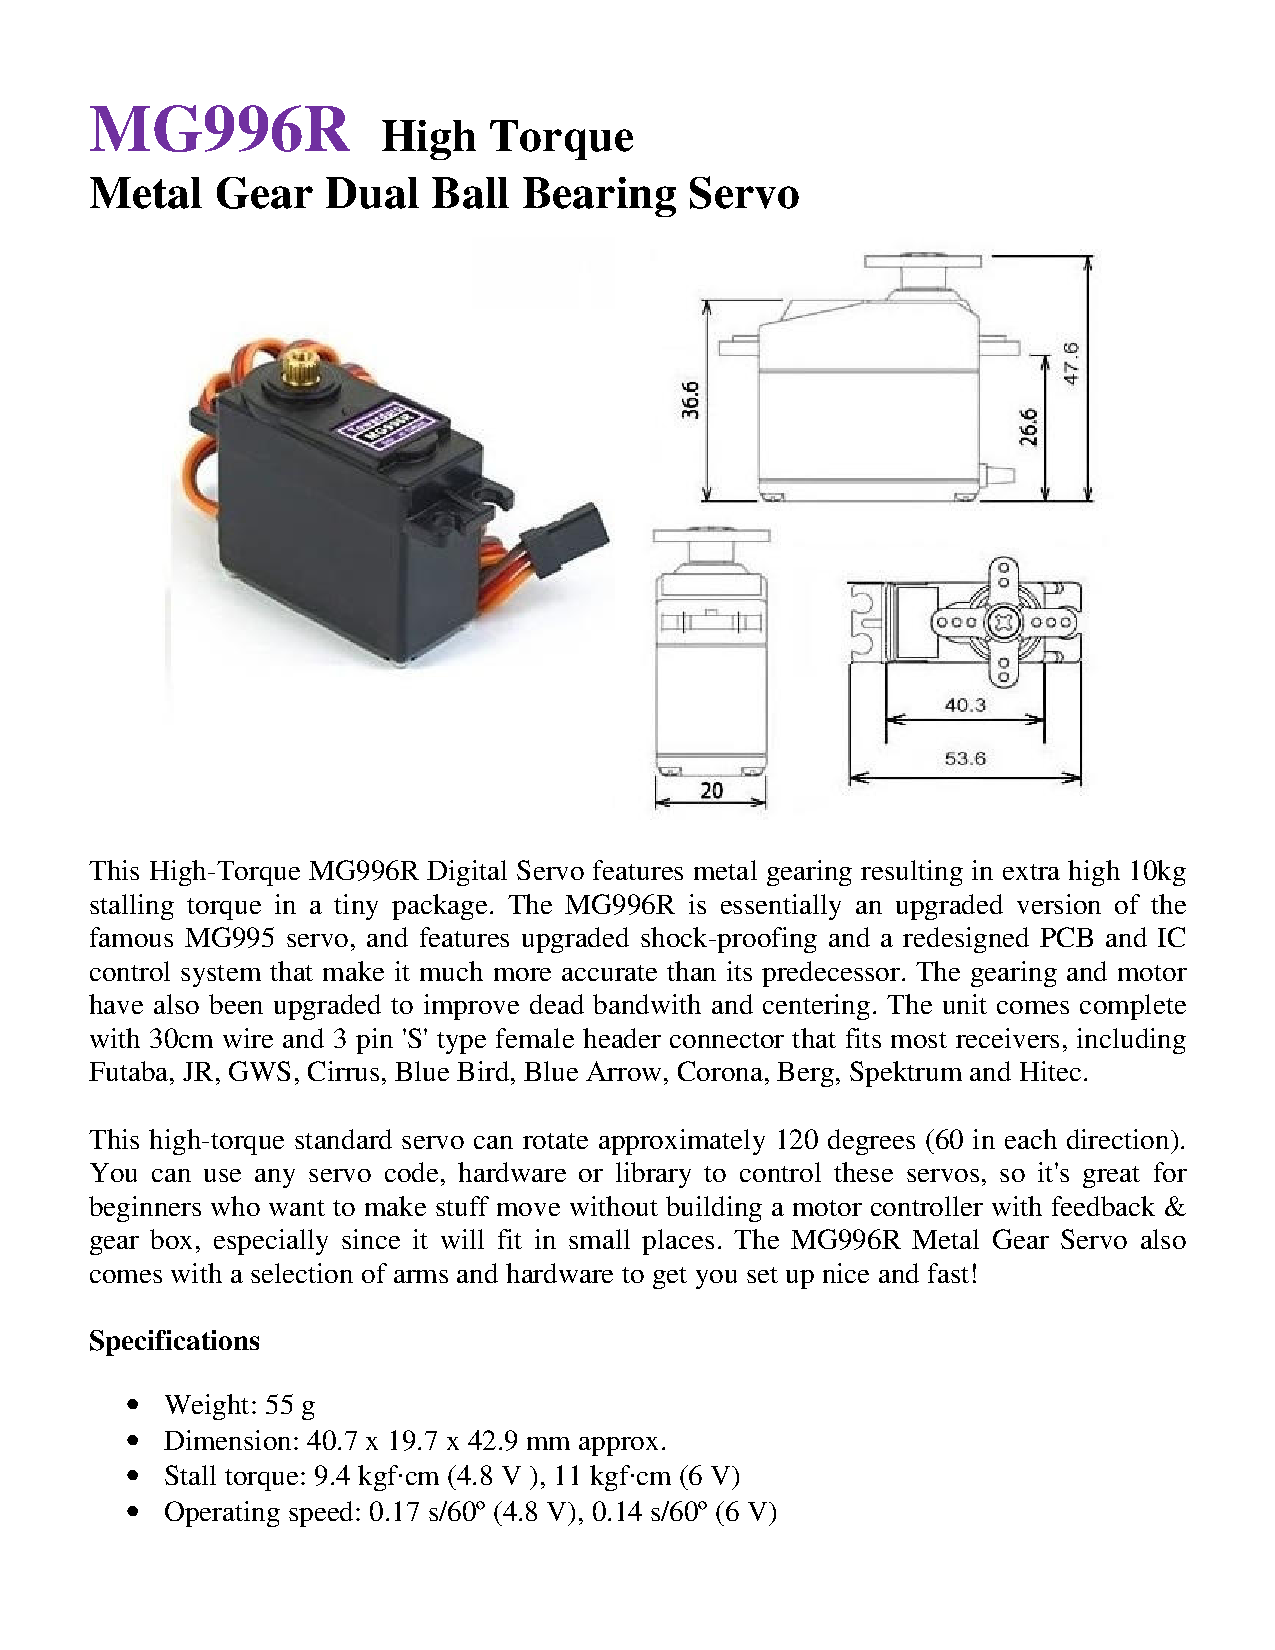
\includepdf[pages=-,fitpaper]{datasheet/MG996R.pdf}

\end{document}